\pdfoutput=1
\pdfcompresslevel=9 
\pdfinfo     
{  
    /Author (Wojciech Klicki,Konrad Starzyk)
    /Title ()
    /Subject (Integracja system�w mobilnych) 
    /Keywords (Integracja mobilna, Systemy Enterprise) 
} 
%\documentclass[a4paper,polish,onecolumn,oneside,floatssmall,11pt,titleauthor,wide,openright]{mwrep}
%\usepackage[scale={0.7,0.8},paper=a4paper,twoside]{geometry}

\documentclass[a4paper,polish,onecolumn,oneside,11pt,wide,floatssmall]{mwrep}
\usepackage{polish} 
\usepackage{amsmath}     
\usepackage{amsfonts}     
%\usepackage{amssymb}  
\usepackage{amsthm}         
\usepackage{bookman}  
\usepackage{fancyhdr}     
\usepackage[cp1250]{inputenc}  
\usepackage{makeidx}   
\makeindex 

\usepackage{geometry}
\usepackage{t1enc}
% \usepackage[pdftex, bookmarks]{hyperref}
\usepackage[pdftex, bookmarks=false, hyperref=false]{hyperref}
\def\url#1{{ \tt #1}}

\usepackage{listings}
  
% marginesy
\textwidth\paperwidth
\advance\textwidth -65mm %reguluje prawy margines
\oddsidemargin-0.9in
\advance\oddsidemargin 33mm
\evensidemargin-0.9in
\advance\evensidemargin 33mm 
\topmargin -1in
\advance\topmargin 25mm
\setlength\textheight{45\baselineskip} %ilosc linii - pozwala na regulacje
									   %dolngo marginesu
\addtolength\textheight{\topskip}
\marginparwidth15mm

\clubpenalty=10000 % to kara za sierotki
\widowpenalty=10000 % nie pozostawia wd�w
\brokenpenalty=10000 % nie dzieli wyraz�w pomi�dzy stronami 
\sloppy

\tolerance4500
\pretolerance250
\hfuzz=1.5pt
\hbadness1450

% �YWA PAGINA 
\renewcommand{\chaptermark}[1]{\markboth{\scshape\small\bfseries \
#1}{\small\bfseries \ #1}}
\renewcommand{\sectionmark}[1]{\markboth{\scshape\small\bfseries\thesection.\
#1}{\small\bfseries\thesection.\ #1}}
\renewcommand{\headrulewidth}{0.5pt}
\renewcommand{\footrulewidth}{0.pt}  
\pagestyle{uheadings}

\usepackage[pdftex]{color,graphicx}

%\usepackage[utf8]{inputenc}
%\usepackage[polish]{babel}

% \textheight232mm
%%% \setlength{\textwidth}{\textwidth}
% \setlength{\oddsidemargin}{\evensidemargin}
% \setlength{\evensidemargin}{0.3cm}
\usepackage[sort, compress]{cite}

%\usepackage{multibib}
%\newcites{bk,st,doc,web}{Ksi��ki i~artyku�y,Standardy i~zalecenia,Dokumentacja produkt�w,Publikacje i~serwisy internetowe}

\theoremstyle{definition}
\newtheorem{defn}{Definicja}[section]
\newtheorem{conj}{Teza}[section]
\newtheorem{conjmain}{Teza}
\newtheorem{exmp}{Przyk�ad}[section]

\theoremstyle{plain}% default
\newtheorem{thm}{Twierdzenie}[section]
\newtheorem{lem}[thm]{Lemat}
\newtheorem{prop}[thm]{Hipoteza}
\newtheorem*{cor}{Wniosek}

\theoremstyle{remark}
\newtheorem*{rem}{Uwaga}
\newtheorem*{note}{Uwaga}
\newtheorem{case}{Przypadek}

\definecolor{ListingBackground}{rgb}{0.95,0.95,0.95}

\begin{document}

% kody �r�d�owe wplatane w tekst
\lstdefinestyle{incode}
{
basicstyle={\footnotesize},
keywordstyle={\bf\footnotesize\color{blue}},
commentstyle={\em\footnotesize\color{magenta}},
numbers=left, 
stepnumber=5, 
firstnumber=1,
numberfirstline=true,
numberblanklines=true,
numberstyle={\sf\tiny}, 
numbersep=10pt, 
tabsize=2,
xleftmargin=17pt,
framexleftmargin=3pt,
framexbottommargin=2pt,
framextopmargin=2pt,
framexrightmargin=0pt,
showstringspaces=true,
backgroundcolor={\color{ListingBackground}},
extendedchars=true,
% title=\lstname,
captionpos=b,
% abovecaptionskip=1pt,
% belowcaptionskip=1pt,
frame=tb,
framerule=0pt, 
}
 
% kody �r�d�owe z podpisem
\lstdefinestyle{outcode}
{
basicstyle={\footnotesize},
keywordstyle={\bf\footnotesize\color{blue}},
commentstyle={\em\footnotesize\color{magenta}},
numbers=left, 
stepnumber=5, 
firstnumber=1,
numberfirstline=true,
numberblanklines=true,
numberstyle={\sf\tiny}, 
numbersep=10pt, 
tabsize=2,
xleftmargin=17pt,
framexleftmargin=3pt,
framexbottommargin=2pt,
framextopmargin=2pt,
framexrightmargin=0pt,
showstringspaces=true,
backgroundcolor={\color{ListingBackground}},
extendedchars=true,
% title=\lstname,
captionpos=b,
% abovecaptionskip=1pt,
% belowcaptionskip=1pt,
frame=tb,
framerule=0.1pt, 
}

\renewcommand*\lstlistingname{Wydruk}
\renewcommand*\lstlistlistingname{Spis wydruk�w}

\pagenumbering{roman}
\renewcommand{\baselinestretch}{1.0}
\raggedbottom

\begin{titlepage}
    % Strona tytu�owa
    \vbox to\textheight{\hyphenpenalty=10000
    \begin{center}
	\begin{tabular}{p{107mm} p{9cm}}
	    \begin{minipage}{9cm}
	      \begin{center}
	      Politechnika Warszawska \\
	      Wydzia�� Elektroniki i~Technik Informacyjnych \\
	      Instytut Informatyki
	      \end{center}
	    \end{minipage}
	    &
	    \begin{minipage}{8cm}
	    \begin{flushleft}
	     \footnotesize
	      Rok akademicki 2008/2009
	    \vspace*{2.75\baselineskip}
	    \end{flushleft}
	    \end{minipage} \\
	\end{tabular}
	\vspace*{3.75\baselineskip}
	\par\vspace{\smallskipamount}
	\vspace*{2\baselineskip}{\LARGE Praca dyplomowa magisterska\par}
	\vspace{3\baselineskip}{\LARGE\strut Wojciech Klicki\\Konrad Starzyk\par}
	\vspace*{2\baselineskip}{\huge\bfseries Integracja technologii mobilnych i system�w klasy Enterprise\par}
	
	\vspace*{7\baselineskip}
	\hfill\mbox{}\par\vspace*{\baselineskip}\noindent
	\begin{tabular}[b]{@{}p{3cm}@{\ }l@{}}
	    {\large\hfill } & {\large }
	\end{tabular}
	\hfill
	\begin{tabular}[b]{@{}l@{}}
	Opiekun pracy: \\[\smallskipamount]
	{\large mgr in�. Piotr Salata}
	\end{tabular}\par
	\vspace*{4\baselineskip}
    \begin{tabular}{p{\textwidth}}
    \begin{flushleft}
	\begin{minipage}{7cm}    
	Ocena \dotfill 
	\par\vspace{1.6\baselineskip}
	\dotfill 
	\par\noindent
	\centerline{\footnotesize Podpis Przewodnicz�cego} \par
	\centerline{\footnotesize Komisji Egzaminu Dyplomowego}\par
	\end{minipage}
    \end{flushleft}
    \end{tabular}
    \end{center}}

    % �yciorys Wojtek
    \newpage\thispagestyle{empty}
    \begin{tabular}{p{5cm} p{12cm}}
    \begin{minipage}{5cm}
    \center
    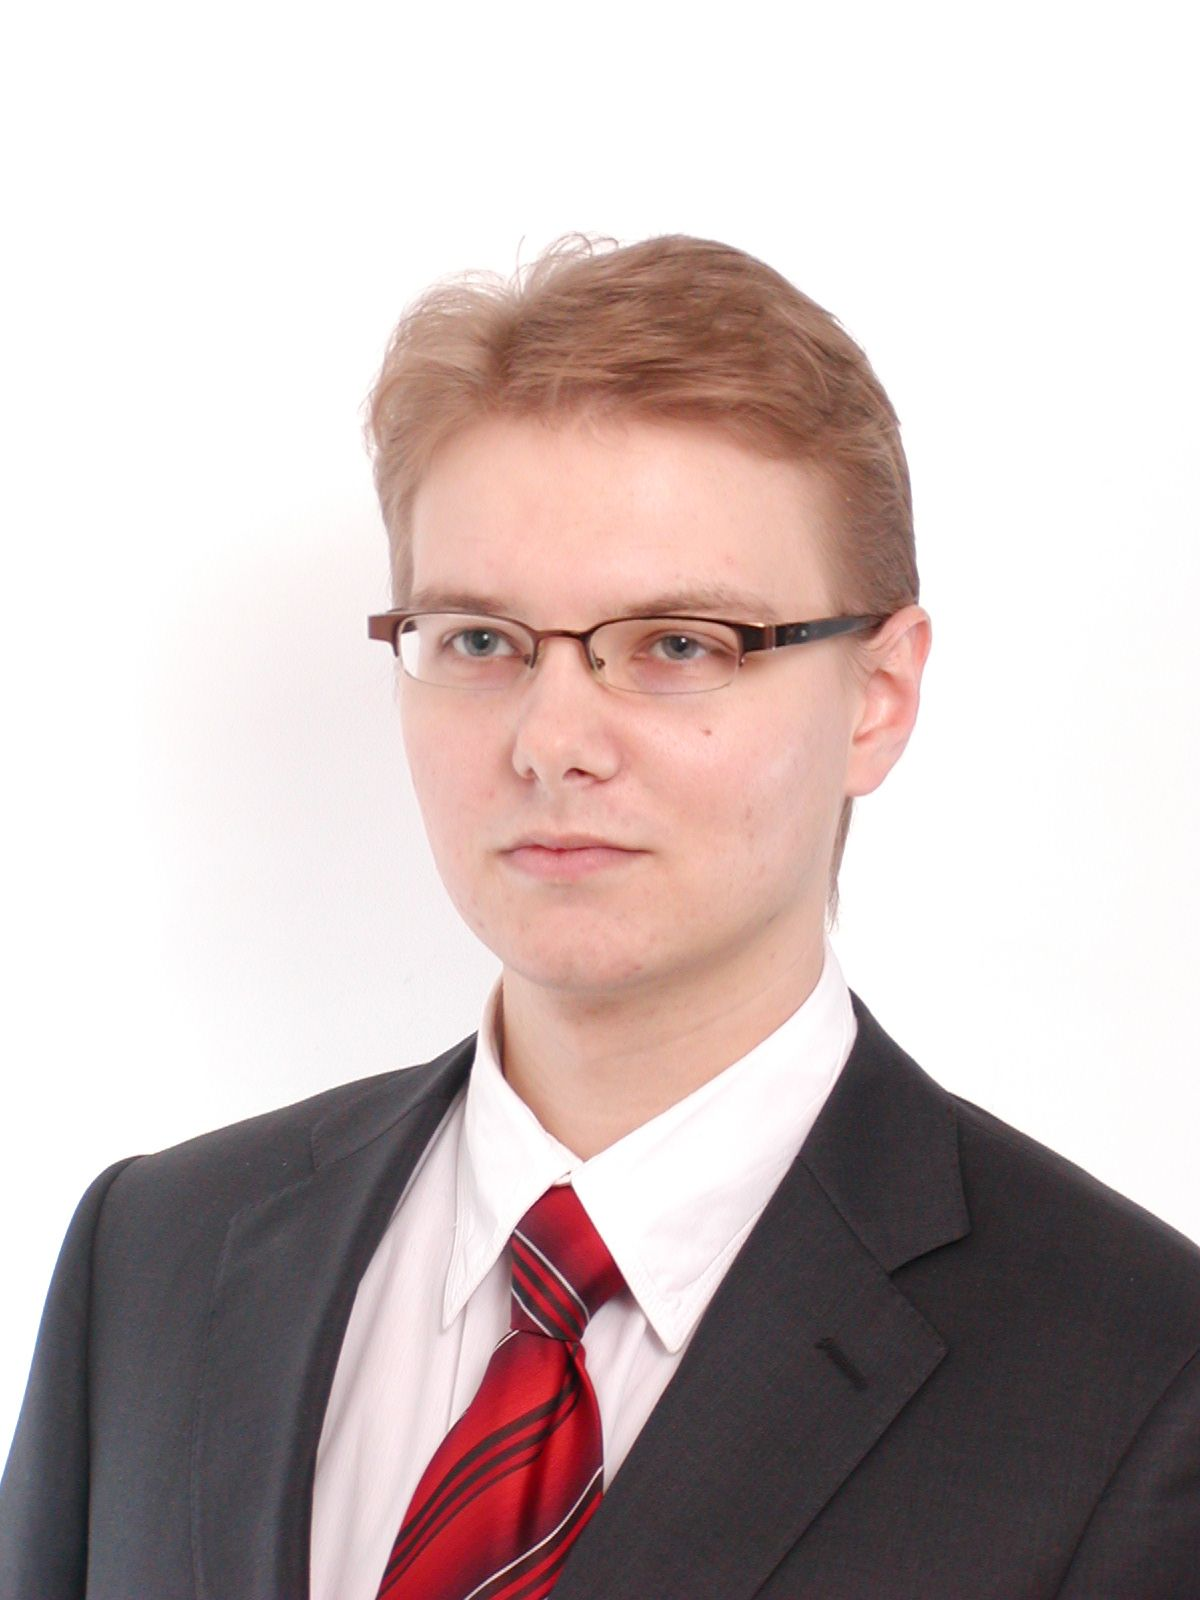
\includegraphics[height=6.5cm,width=4.5cm]{img/wojtek.jpg} 
    \end{minipage}
    &
    \begin{minipage}{12cm}
    \begin{flushleft}
    \par\noindent\vspace{1\baselineskip} 
    \begin{tabular}[h]{l l}
    {\normalsize\it Specjalno��:} & In�ynieria System�w Informacyjnych 
    \end{tabular}
    \par\noindent\vspace{1\baselineskip} 
    \begin{tabular}[h]{l l}
    {\normalsize\it Data urodzenia:} & {\normalsize 8 pa�dziernika 1984~r.} 
    \end{tabular}
    \par\noindent\vspace{1\baselineskip}
    \begin{tabular}[h]{l l}
    {\normalsize\it Data rozpocz�cia studi�w:} & {\normalsize 23 lutego
    2008 r.}
    \end{tabular}
    \par\noindent\vspace{1\baselineskip}
    \end{flushleft}
    \end{minipage}
    \end{tabular}
    \vspace*{1\baselineskip}
    \begin{center}
	{\large\bfseries �yciorys}\par\bigskip
    \end{center}
    
    \indent
    
  Urodzi�em sie 8 pa�dziernika 1984 roku w Ciechanowie. Po ukonczeniu szko�y 
podstawowej nr 6 kontynuowa�em nauke w I Liceum Og�lnokszta�c�cym im. Zygmunta 
Krasinskiego w Ciechanowie. W lutym 2004 roku rozpocz��em studia na Wydziale
Elektroniki i Technik Informacyjnych Politechniki Warszawskiej. W lutym 2008 roku uzyska�em
tytu� in�yniera.
    \par
    \vspace{2\baselineskip}
    \hfill\parbox{15em}{{\small\dotfill}\\[-.3ex]
    \centerline{\footnotesize podpis studenta}}\par
    \vspace{3\baselineskip}
    \begin{center}
 	{\large\bfseries Egzamin dyplomowy} \par\bigskip\bigskip
    \end{center}
    \par\noindent\vspace{1.5\baselineskip}
    Z�o�y� egzamin dyplomowy w dn. \dotfill 
    \par\noindent\vspace{1.5\baselineskip}
    Z wynikiem \dotfill 
    \par\noindent\vspace{1.5\baselineskip}
    Og�lny wynik studi�w \dotfill
    \par\noindent\vspace{1.5\baselineskip}
    Dodatkowe wnioski i uwagi Komisji \dotfill
    \par\noindent\vspace{1.5\baselineskip}
    \dotfill
    
    
     % �yciorys Wojtek
    \newpage\thispagestyle{empty}
    \begin{tabular}{p{5cm} p{12cm}}
    \begin{minipage}{5cm}
    \center
    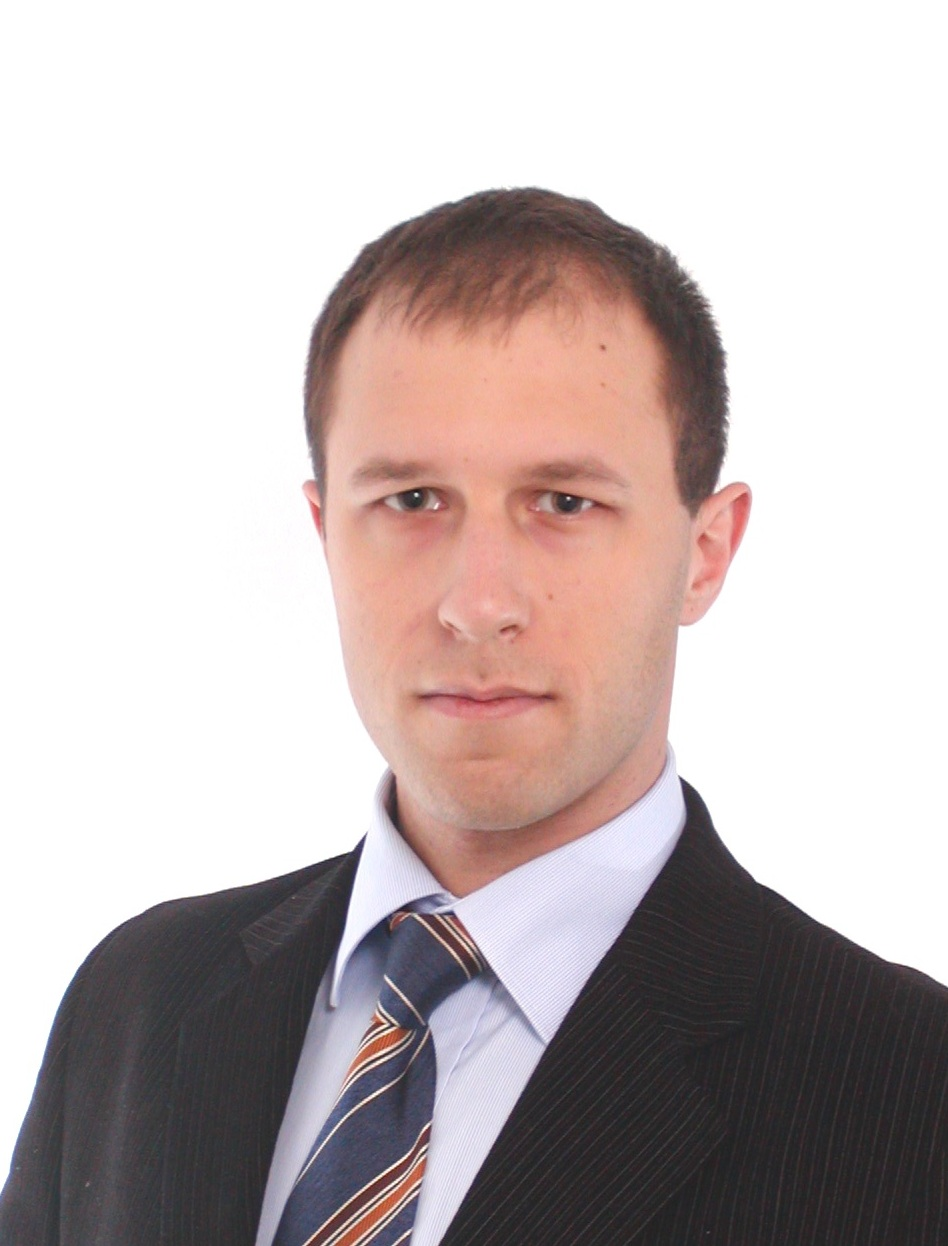
\includegraphics[height=6.5cm,width=4.5cm]{img/konrad_cut.jpg} 
    \end{minipage}
    &
    \begin{minipage}{12cm}
    \begin{flushleft}
    \par\noindent\vspace{1\baselineskip} 
    \begin{tabular}[h]{l l}
    {\normalsize\it Specjalno��:} & In�ynieria System�w Informacyjnych 
    \end{tabular}
    \par\noindent\vspace{1\baselineskip} 
    \begin{tabular}[h]{l l}
    {\normalsize\it Data urodzenia:} & {\normalsize 29 lipca 1984~r.} 
    \end{tabular}
    \par\noindent\vspace{1\baselineskip}
    \begin{tabular}[h]{l l}
    {\normalsize\it Data rozpocz�cia studi�w:} & {\normalsize 23 lutego
    2008 r.}
    \end{tabular}
    \par\noindent\vspace{1\baselineskip}
    \end{flushleft}
    \end{minipage}
    \end{tabular}
    \vspace*{1\baselineskip}
    \begin{center}
	{\large\bfseries �yciorys}\par\bigskip
    \end{center}
    
    \indent
    Urodzi�em sie 29 lipca 1984 roku w Olsztynie. Po ukonczeniu szko�y
    podstawowej nr 6 kontynuowa�em nauke w I Liceum Og�lnokszta�c�cym im.
    Zygmunta Krasi�skiego w Ciechanowie. W lutym 2004 roku rozpocz��em studia
    na Wydziale Elektroniki i Technik Informacyjnych Politechniki Warszawskiej.
    W lutym 2008 roku uzyska�em tytu� in�yniera.
    \par
    \vspace{2\baselineskip}
    \hfill\parbox{15em}{{\small\dotfill}\\[-.3ex]
    \centerline{\footnotesize podpis studenta}}\par
    \vspace{3\baselineskip}
    \begin{center}
 	{\large\bfseries Egzamin dyplomowy} \par\bigskip\bigskip
    \end{center}
    \par\noindent\vspace{1.5\baselineskip}
    Z�o�y� egzamin dyplomowy w dn. \dotfill 
    \par\noindent\vspace{1.5\baselineskip}
    Z wynikiem \dotfill 
    \par\noindent\vspace{1.5\baselineskip}
    Og�lny wynik studi�w \dotfill
    \par\noindent\vspace{1.5\baselineskip}
    Dodatkowe wnioski i uwagi Komisji \dotfill
    \par\noindent\vspace{1.5\baselineskip}
    \dotfill

    % Streszczenie
    \newpage\thispagestyle{empty}
    \vspace*{2\baselineskip}
    \begin{center}
	{\large\bfseries Streszczenie}\par\bigskip
    \end{center}
    
    {\itshape 
    Praca ta prezentuje zagadnienia zwi�zane z integracj� system�w klasy
    enterprise i urz�dze� mobilnych. Przedstawione zosta�y rodzaje integracji,
     problemy, kt�re nale�y rozwa�y� oraz istniej�ce podej�cia do tworzenia aplikacji mobilnych.
      W cz�ci implementacyjnej pracy zaproponowany zosta� szablon integracyjny
      dla urz�dze� mobilnych wraz z przyk�adow� implementacj�. } \vspace*{1\baselineskip}
    
    \noindent{\bf S�owa kluczowe}: {\itshape integracja, urz�dzenia mobilne,
    enterprise, webserwisy, wiadomo�ci, jms, kuix, blackberry, symbian, opera
    mini, internet explorer mobile}
    \par
    \vspace{4\baselineskip}
    \begin{center}
	{\large\bfseries Abstract}\par\bigskip
    \end{center}
    \noindent{\bf Title}: {\itshape Mobile devices to
    enterprise-class systems integration 
     }\par \vspace*{1\baselineskip} {\itshape This thesis presents issues connected
    with mobile devices to enterprise integration. Different kinds of 
    integration have been shown, along with integration challenges that ought to
    be considered. Furthermore, various approaches of mobile applications
    development are described. Finally, in the implementation part, a sample
    integration framework and its appliance is presented.
    } \vspace*{1\baselineskip}
       
    \noindent{\bf Key words}: {\itshape integration, mobile devices,
    enterprise, webservices, messages, jms, kuix, blackberry, symbian, opera
    mini, internet explorer mobile}
   
\end{titlepage}

% ex: set tabstop=4 shiftwidth=4 softtabstop=4 noexpandtab fileformat=unix filetype=tex encoding=utf-8 fileencodings= fenc= spelllang=pl,en spell:



\linespread{1.5}%
\selectfont 

\tableofcontents
% \addcontentsline{toc}{chapter}{{Przedmowa1}{vii}}{vii}

% \chapter*{Spis tablic, rysunk�w i~wydruk�w}
% \listoftables
% \listoffigures
% \lstlistoflistings 

%\setlength{\baselineskip}{7mm}
\newpage
\pagenumbering{arabic}
\setcounter{page}{1}


\chapter{Integracja w �rodowiskach Enterprise} 
 Oprogramowanie Enterprise jest poj�ciem do�� szerokim, opisuj�cym systemy
przeznaczone dla przedsi�biorstw. Programy, wchodz�ce w sk�ad tych system�w,
odwzorowuj� zachodz�ce procesy biznesowe. Niekiedy poj�cie Enterprise odnosi
si� do oprogramowania pisanego na zam�wienie. Mo�e te� odnosi� si� do
rozbudowanych pakiet�w wspieraj�cych okre�lone czynno�ci. Jako przyk�ad
mo�na przytoczy� kontakty z klientami lub ksi�gowo��. Jednak rzadko si� zdarza,
by istnia� jeden system, kt�ry potrafi�by spe�ni� wymagania klienta. Gdyby  
nawet istnia�by taki program, to firma z r�nych przyczyn mo�e nie chcie� go
wdro�y�. Tak wi�c nawet w obr�bie jednego przedsi�biorstwa cz�sto mo�na
spotka� si� z sytuacj�, w kt�rej dzia�a wiele niezale�nych aplikacji. Nierzadko
s� one pisane przez r�ne firmy. Pomi�dzy wspomnianymi aplikacjami zachodzi
potrzeba komunikacji, na przyk�ad w celu wymiany danych. Wraz z realizacj� tej
potrzeby pojawiaj� si� pewne sta�e problemy. Zostan� one opisane w niniejszej
pracy, gdy� ich rozwi�zywanie jest najwa�niejszym elementem procesu integracji.
\newline
Jeszcze do niedawna m�wi�c o integracji mieli�my na my�li wy��cznie serwery
aplikacyjne. Obecnie obowi�zuj�cym trendem jest post�puj�ca miniaturyzacja i
wzrost mocy obliczeniowej urz�dze� mobilnych udost�pniaj�cych klientom
us�ugi, dost�pne do tej pory wy��cznie za po�rednictwem komputera
stacjonarnego. Tworz�c aplikacj� na urz�dzenia przeno�ne, kt�ra b�dzie wsp�pracowa�a z
istniej�cymi ju� systemami, napotykamy na nowe problemy wynikaj�ce ze
specyfiki �rodowiska mobilnego.

\section{Potrzeba integracji}

Potrzeba integracji pojawia si�, gdy pojawia si� r�norodno��, kt�ra
wymaga dodatkowego nak�adu pracy sprowadzaj�cego j� do wsp�lnego poziomu.
Warto zauwa�y�, �e istniej� r�ne poziomy r�norodno�ci, a
rozwi�zania integracyjne mog� albo usuwa� t� r�norodno�� na poziomie
technicznym albo odpowiada� na potrzeby wynikaj�ce z r�norodno�ci na wy�szym
poziomie, na przyk�ad organizacyjnym. Mo�emy wi�c wyr�ni� nast�puj�ce poziomy
r�norodno�ci:
\begin{itemize}
  \item Infrastrukturalna
  \subitem - u�ycie r�nych narz�dzi i architektur
  \subitem - u�ycie r�nych standard�w i proces�w
  \item Dyscyplinarna
  \subitem  - oddzielne dzia�y wewn�trz firmy lub r�ne firmy
  \item Geograficzna
  \subitem - w ramach jednego kraju
  \subitem - w ramach wielu kraj�w/stref czasowych
  \item Zawarto�ci
  \subitem - rozdzielenie dzia��w operacyjnych, np. obs�uga klienta, logistyka,
  ksi�gowo��
  \subitem - podzia� pracy pomi�dzy dzia�y, np procesu kt�ry jest obs�ugiwany
  przez ka�dy z nich
\end{itemize}

W niniejszej pracy nie b�dziemy rozwa�a� przyczyn r�norodno�ci, przyjmujemy j�
raczej jako problem, kt�ry nale�y rozwi�za�. Jednak samo zwr�cenie uwagi
na list� mo�liwych przyczyn, sprawia, �e mo�emy sobie wyobrazi�, i� systemy
jakie spotykamy w przedsi�biorstwach du�ej skali cz�sto sk�adaj� si� z setek, je�li nie tysi�cy aplikacji wykonanych na zam�wienie przez zewn�trzne firmy lub przez wewn�trzne dzia�y informatyczne. Cz�� z tych aplikacji jest
tak zwanymi 'legacy systems' napisanymi w zapomnianych ju� j�zykach,
przygotowanymi pod platformy, kt�re cz�sto nie mog� liczy� ju� na wsparcie
producent�w. Wielokrotnie mo�na natrafi� na kombinacje tego typu aplikacji
dzia�aj�ce w r�nych warstwach w obr�bie r�nych system�w operacyjnych.

\subsection{Pe�nowarto�ciowe �rodowiska informatyczne}

Przyczyn le��cych u podstaw tak du�ego skomplikowania sytuacji w �rodowiskach
informatycznych typu Enterprise nale�y doszukiwa� si� w skomplikowaniu
zagadnienia jakim jest projektowanie du�ych aplikacji. Zbudowaniem jednej, posiadaj�cej
wszystkie niezb�dne funkcje aplikacji, kt�ra by�aby w stanie w pe�ni zaspokoi�
potrzeby du�ego przedsi�biorstwa. Firmy dzia�aj�ce na rynku ERP (Enterprise
Resource Planning) od lat nie ustaj� w wysi�kach by zbudowa� tego typu
aplikacj�. Jednak nawet najwi�ksze z nich wytworzy�y produkty, kt�re pokrywaj�
tylko cz�� niezb�dnych funkcji. Mo�na to zaobserwowa� na przyk�adzie system�w,
kt�re stanowi� punkty integracyjne we wsp�czesnych rozwi�zaniach.
Kolejnym powodem jest to, �e rozwi�zania, kt�re sk�adaj� si� z wielu ma�ych
zintegrowanych podsystem�w pozwalaj� na pewn� elastyczno�� w doborze
najlepszych rozwi�za� w zakresie danej dziedziny. Mog� wybra� takie
rozwi�zanie, kt�re jest w danej chwili najlepsze i stosunkowo najta�sze na
rynku. Nie s� zmuszeni do inwestowania w ca�o�ciowe rozwi�zania dostarczane
przez tylko jednego dostawc�. Co wi�cej opieranie si� na wielu podsystemach
wykonywanych przez r�ne firmy mo�e pozwoli� na pewne zr�wnoleglenie prac nad
wdro�eniem odr�bnych cz�ci systemu. W przypadku jednego du�ego systemu
potencjalnie prace nad nim mog�yby by� blokowane przez braki w zasobach
przedsi�biorstwa realizuj�cego zlecenie wdro�enia.\newline
Niestety takie podej�cie przynosi najlepsze efekty przy �cis�ym podziale
funkcjonalno�ci pomi�dzy produktami r�nych producent�w. W rzeczywisto�ci
pokusa budowania system�w, kt�re zabior� elementarn� funkcjonalno�� innej
cz�ci z zupe�nie innego pola, jest zbyt du�a i prowadzi do powstawania
rozwi�za�, kt�re nie maj� wyra�nego podzia�u na dziedziny.\newline
Przy rozwi�zaniach tego typu nale�y zwr�ci� uwag�, �e z punktu widzenia
u�ytkownika system enterprise, pomimo �e w rzeczywisto�ci mo�e sk�ada� si� z
wielu ma�ych, zintegrowanych ze sob� system�w, stanowi jedn� ca�o��. Na
przyk�ad u�ytkownik mo�e wys�a� zapytanie o stan konta oraz adres zamieszkania
klienta. W sytuacji gdy mamy do czynienia z systemem korporacyjnym takie
zapytanie mo�e wymaga� odwo�ania si� do dw�ch zupe�nie r�nych podsystem�w
(bilingowego oraz kontaktu z klientem). System cz�sto musi dokona� autentykacji
oraz autoryzacji u�ytkownika, sprawdzi� obci��enie serwer�w w celu wybrania
optymalnego do realizacji zlecenia. Tego typu proces mo�e w bardzo prosty
spos�b zaanga�owa� kilka system�w. Z punktu widzenia u�ytkownika jest to
pojedyncza transakcja.\newline
W celu zapewnienia poprawno�ci dzia�ania system�w, umo�liwienia wydajnej
wymiany danych oraz zapewnienia przezroczystego funkcjonowania proces�w
biznesowych, opisane powy�ej aplikacje musz� zosta� zintegrowane. Wraz z
integracj� pojawiaj� si� inne potrzeby takie jak zapewnienie bezpiecznej
wymiany danych czy te� umo�liwienie dost�pu do systemu z r�nych platform
zewn�trznych.

\subsection{Systemy mobilne}

Jedn� z podstawowych cech jakie musi posiada� system enterprise jest �atwo��
dost�pu do przechowywanym w nim informacji. Typowy u�ytkownik takiego systemu
chce mie� mo�liwo�� po��czenia si� z nim i pobrania konkretnych informacji o
ka�dej porze dnia czy nocy. Wraz z pojawieniem si� nowej generacji urz�dze�
mobilnych mo�liwym sta�o si� zrealizowanie tej potrzeby. Nowoczesne platformy
oferuj� niespotykan� wcze�niej moc oraz zasi�g, kt�re pozwalaj� na sta�y dost�p
do sieci firmowej z dowolnego niemal miejsca na ziemi. Us�ugi synchronizuj�ce
poczt� korporacyjn�, oferuj�c� pojedyncz� skrzynk� poczty przychodz�cej, s�
obecnie niezb�dnym minimum w ka�dej du�ej firmie. Nast�pnym etapem w rozwoju
jest umo�liwianie szybkiego i interaktywnego dost�pu do dzia�aj�cych w obr�bie
intranetu us�ug wewn�trznych. Ten nowy rodzaj potrzeby integracji - integracja
mobilna, stanowi zupe�nie nowy rodzaj wyzwania dla firm oferuj�cych narz�dzia
dla biznesu. Niesie ona ze sob� zupe�nie nowe zagadnienia oraz problemy, kt�re
nie by�y spotykane przy klasycznej integracji. Wymusza to wypracowanie zupe�nie
nowej metodologii przemys�owego wytwarzania oprogramowania zapewniaj�cego
zaspokojenie tej potrzeby.
  
\section{Klasyczne wyzwania integracji}

Integracja aplikacji w przedsi�biorstwach cz�sto nie jest prostym zadaniem.
Mimo, �e w niemal ka�dej du�ej firmie zachodzi potrzeba integracji i powsta�o
ju� wiele opracowa� na ten temat, nikt nie przedstawi� kompletnej listy
problem�w, kt�re nale�a�oby rozwa�y� podczas integrowania system�w. Dodatkowo,
wyzwania, kt�re stawia integracja, wykraczaj� nie tylko poza techniczne
rozwa�ania, ale tak�e rozci�gaj� si� na procedury biznesowe. Tak jak ju�
wspominali�my, przedstawienie kompletnej listy takich problem�w nie jest
mo�liwe ze wzgl�du na konieczno�� dokonania analizy ka�dego z przypadk�w. Mimo to spr�bujemy
przedstawi� te najbardziej typowe w wi�kszo�ci opisane w \cite{Entpatterns},
kt�re koniecznie trzeba wzi�� pod uwag�:

\subsection{Wyzwania techniczne}

\paragraph{Fizyczna i logiczna odr�bno�� system�w,}
z kt�rej tak naprawd� wynika potrzeba integracji. Wprowadza to jednak konieczne
do rozwa�enia kwestie, takie jak:
\begin{itemize}
  \item wyb�r sposobu komunikacji mi�dzy systemami (o kt�rych wi�cej w
  rozdziale 1.4)
  \item wp�yw tego wyboru na bezpiecze�stwo i zgodno�� takiego rozwi�zania z
  polityk� bezpiecze�stwa firmy
\end{itemize}
  
\paragraph{Ograniczony dost�p do integrowanych aplikacji.}
Cz�sto okazuje si�, �e integrowane aplikacje to istniej�ce od dawna systemy,
kt�re nie do��, �e nie daj� mo�liwo�ci zmian w �r�d�ach, to dodatkowo
udost�pniaj� mocno ograniczony interfejs zewn�trzny. W takiej sytuacji
programi�ci musz� niekiedy ucieka� si� do stosowania niskopoziomowych
modyfikacji (np. na bazie danych, kt�rej u�ywa aplikacja) czy w ostateczno�ci
do dekompilacji jej modu��w.


\paragraph{Brak uniwersalnego standardu wymiany danych pomi�dzy aplikacjami.}
Pomimo �e problemy z komunikacj� przy integracji danych znane s� od wielu lat,
du�a cz�� aplikacji nie wspiera �adnego uniwersalnego formatu danych, co
powoduje konieczno�� specjalizowania platform integracyjnych pod k�tem
pod��czanych do niej aplikacji. Jako rozwi�zanie tego problemu cz�sto stosuje
si� XML i Web serwisy. Jednak wsparcia dla ich obs�ugi mo�emy oczekiwa�
jedynie w przypadku stosunkowo nowych aplikacji. Nawet te technologie nie daj�
gwarancji pe�nej uniwersalno�ci ze wzgl�du na dodatkowe rozszerzenia, kt�re si�
wykszta�ci�y w ramach Web serwis�w (o kt�rych wi�cej informacji w dalszej
cz�ci pracy). Warto zauwa�y�, �e ten sam problem - brak wsp�pracy pomi�dzy
aplikacjami oficjalnie wspieraj�cymi pewien standard - by� g��wn� przeszkod� w
stosowaniu CORBY - zaawansowanego protoko�u, umo�liwiaj�cego wsp�prac�
aplikacji stworzonych w r�nych j�zykach i dzia�aj�cych na r�nych platformach.
\index{platforma integracyjna}
\paragraph{Utrzymanie platformy integracyjnej.} O ile uruchomienie platformy
integracyjnej - systemu komunikuj�cego ze sob� wiele r�norodnych aplikacji -
jest trudnym zadaniem, o tyle utrzymanie go mo�e by� jeszcze trudniejsze.
Rzadko zdarza si�, by by�a ona ca�kowicie scentralizowana i nie wymaga�a
ingerencji lub chocia� konfiguracji integrowanych aplikacji. W zwi�zku z
powy�szym, osoby, kt�re odpowiadaj� za utrzymanie takiej platformy, musz�
posiada� wiedz� na ich temat. Dodatkowo, ci�ko jest t� wiedz� utrzyma�,
zw�aszcza gdy pracownicy cz�sto si� zmieniaj�. Natura platformy
integracyjnej wymusza jej automatyzacj�, co powoduje, �e mo�e ona
bezproblemowo dzia�a� bardzo d�ugo, wr�cz przezroczy�cie dla wszystkich a� do
wyst�pienia pierwszego problemu lub potrzeby wprowadzenia modyfikacji. 
Wtedy w�a�nie od os�b odpowiedzialnych za platform� integracyjn� wymaga si�
wprowadzenia w niej modyfikacji lub usuni�cia b��d�w. Poniewa� platforma
 jest najcz�ciej centralnym punktem komunikacyjnym, kt�ry
obs�uguje wiele system�w, za ka�dym razem gdy dochodzi do zmian w jednym z
nich, mo�e (cho� oczywi�cie, nie musi) zaj�� potrzeba zmian w platformie
integracyjnej. Takie ryzyko nie istnieje, je�eli integrujemy ze sob� wy��cznie
systemy, kt�re maj� ze sob� wsp�pracowa� (z pomini�ciem punktu centralnego). W
takiej sytuacji, to administratorzy ka�dego z integrowanych system�w wsp�pracuj� ze sob�.
Oczywi�cie, to platforma integracyjna jest rozwi�zaniem bardziej elastycznym,
ale jej utrzymanie bez w�tpienia stanowi du�e obci��enie dla dzia�u IT.
\index{�r�d�o danych}

\paragraph{R�norodno�� �r�de� danych.} Niekiedy pojawia si� potrzeba
integrowania danych, pochodz�cych z r�nych, czasami bardzo nietypowych
�r�de�. 
Przyk�ad mo�e stanowi� wypowied� Hans-Joachim Poppa, szefa Deutsches Zentrum
f�r Luft- und Raumfahrt (Niemieckie Centrum Lotnictwa). W \cite{computerwoche}
opisuje on jak pojawi�o si� rozporz�dzenie nak�adaj�ce konieczno��
gromadzenia w uporz�dkowany spos�b wszystkich danych zwi�zanych z prowadzonymi projektami
naukowymi. Jak m�wi, by�o to trudniejsze ni� mog�oby si� wydawa�. W czasie
realizacji projektu naturalne by�o przesy�anie informacji za pomoc� poczty
elektronicznej jak i organizacja spotka�, na kt�rych powstawa�y notatki. Nie s�
to uporz�dkowane sposoby przesy�ania informacji, co gdy rozporz�dzenie wesz�o w �ycie, 
wprowadzi�o konieczno�� uporz�dkowania i (co jeszcze trudniejsze)
zlokalizowania danych, rozproszonych mi�dzy komputery u�ytkownik�w.

\subsection{Wyzwania biznesowe}

\paragraph{Zmiana polityki wewn�trznej przedsi�biorstwa.} 
Poprawna integracja oznacza nie tylko doprowadzenie do wsp�pracy system�w
informatycznych, ale r�wnie� departament�w w firmie. Wynika to z faktu, �e
integrowane aplikacje najcz�ciej komunikuj� si� automatycznie, co powoduje, �e
wprowadzenie zmian do systemu przez jeden departament mo�e mie� konsekwencje
(np. w postaci realizacji zlecenia) w drugim. Konieczne jest u�wiadomienie
u�ytkownik�w o tym fakcie, tak by integracja przynosi�a korzy�ci w postaci
uproszczenia przep�ywu danych i zaoszcz�dzenia czasu, zamiast pr�b r�cznego
kontrolowania niezale�nych do tej pory aplikacji.

\paragraph{Wp�yw integracji na przedsi�biorstwo.} 
Rozwi�zania integracyjne ��cz� ze sob� wiele aplikacji, kt�rych dzia�anie jest
kluczowe dla funkcjonowania przedsi�biorstwa. Powoduje to, �e b��dy w dzia�aniu
lub niedost�pno�� platformy integracyjnej maj� bardzo powa�ne konsekwencje,
tak�e finansowe. Z drugiej strony, poprawnie funkcjonuj�ca integracja
przyspiesza przep�yw informacji i powoduje, �e ka�dy scenariusz wsp�pracy przebiega w
daj�cych si� przewidzie� krokach, co gwarantuje powtarzalno�� i wiedz� o stanie
wsp�pracy (np. stanie zlecenia, kt�re wp�yn�o i jest obs�ugiwane). Nale�y
pami�ta�, �e utrzymywanie platformy integracyjnej wymaga kontaktu pomi�dzy
osobami opiekuj�cymi si� integrowanymi systemami, a dzia�em utrzymuj�cym
platform�. Nie mo�na dopu�ci� do niekonsultowanych wcze�niej zmian w
kt�rymkolwiek z system�w, gdy� inaczej mo�e to doprowadzi� do awarii wszystkich
integrowanych system�w.


\paragraph{R�nice semantyczne w poj�ciach.} Cho� XML rozwi�zuje wiele problem�w
technicznych, to nie stanowi on odpowiedzi na r�n� semantyk�.
We�my za przyk�ad s�owo "konto". W jednym systemie mo�e oznacza�
numer konta bankowego. Natomiast w innym mo�e to by� wewn�trzny numer
konta w korporacji, czy te� konto u�ytkownika. 
Innym, pokrewnym problemem jest r�ny format zapisu tych samych danych.
Wyobra�my sobie system nawigacji satelitarnej na urz�dzeniu mobilnym po��czony z
bankiem map. Dane otrzymywane z odbiornika GPS s� wsp�rz�dnymi geograficznymi w pewnym uk�adzie
odniesienia. Uk�ad�w odniesienia jest na �wiecie kilkaset i s�u�� one uzyskaniu
jak najwi�kszej dok�adno�ci w danym obszarze. Przyk�adowo, wg \cite{omapach} w
Polsce u�ywany jest uk�ad Pu�kowo 42. Je�eli w odbiorniku GPS
ustawimy uk�ad odniesienia na najpopularniejszy WGS84, to pracuj�c z mapami w
uk�adzie Pu�kowo 42 otrzymamy niedok�adno�� rz�du 6'' czyli oko�o 120m. Cho�
wi�c, u�ywamy wsp�rz�dnych geograficznych do okre�lenia po�o�enia na mapie i w
terenie, rozbie�no�ci, o ile nie uwzgl�dnimy uk�adu odniesienia mog� by� bardzo
znaczne.\\
\indent
Dlatego w�a�nie, w integracji, opr�cz znalezienia wsp�lnych poj��, konieczne
jest sprawdzenie czy pochodz� z tej samej dziedziny, a je�eli tak, to czy maj�
to samo znaczenie. W tym celu przed rozpocz�ciem integracji, powinni�my
przygotowa� s�ownik poj�� zawieraj�cy dok�adne definicje w celu unikni�cia
nieporozumie�. 


\section{Problemy integracji mobilnej}
 \section{Istniej�ce podej�cia do integracji}
Istnieje kilka powszechnie znanych sposob�w integracji, kt�re maj� swoje mocne i
s�abe strony. Mo�na zauwa�y�, �e pojawia�y si� one wraz z rozwojem system�w
informatycznych i ka�dy z nich odpowiada jakiemu� etapowi rozwoju (np.
istnienie plik�w jako podstawowych struktur przechowuj�cych dane na d�ugo przed
pojawieniem si� baz danych). Mimo to, ka�dy z nich ci�gle znajduje swoje
zastosowanie, gdy okazuje si�, �e nie wszystkie mechanizmy s� jednakowo
dost�pne, lub, gdy bardziej skomplikowane technologie wprowadzaj� zbyt du�y
narzut.

\paragraph{Transfer plik�w}- jedna aplikacja zapisuje plik w okre�lonym
formacie w ustalonym miejscu, nast�pnie druga go odczytuje i przetwarza. Zalet�
takiego rozwi�zania jest jego dost�pno�� - prawie zawsze b�dziemy mieli
dost�p do systemu plik�w. Poza tym nie musimy wiedzie�, jak dzia�a
aplikacja. Jedyne, co powinni�my zrobi�, to dostarczy� plik we w�a�ciwym
formacie. Z drugiej strony, nie istnieje �aden spos�b wymuszenia formatu
zapisywanego pliku. Mo�emy zapisa� na dysku dowolny plik, a aplikacja
docelowa b�dzie go mog�a ewentualnie odrzuci�.
    
\paragraph{Wsp�lna baza danych}- dwie aplikacje dzia�aj� na jednej bazie
danych. W momencie, gdy obie korzystaj� z tych samych danych, to nie ma potrzeby
ich duplikacji. Dodatkowo, przez ograniczenia wymuszone przez baz�, musimy
je zapisywa� w �ci�le okre�lonym formacie, przestrzegaj�c typ�w i wi�z�w
integralno�ci. Niestety, trudno jest tak� baz� zaprojektowa�. Gdyby�my
nawet stworzyli dwie takie aplikacje, kt�re wsp�pracuj� z jedn� baz� danych,
to w wypadku, gdyby�my chcieli do��czy� kolejn�, wsp�pracuj�c� aplikacj�,
mog�oby si� to wi�za� z konieczno�ci� przemodelowania bazy danych. Dodatkowo,
zmiana danych w bazie nie zawsze wystarczy. Mo�emy sobie wyobrazi� sytuacj�,
w kt�rej zmiana wysoko�ci pensji niesie za sob� konieczno�� wykonania
dodatkowych czynno�ci, np. zmiany wysoko�ci sk�adki w systemie
ubezpieczeniowym.
	
\paragraph{Zdalne wywo�ywanie procedur}- mo�e si� odbywa� z
wykorzystaniem mechanizm�w typowych dla danej technologii (RPC,RMI czy
WebServices). Jedna aplikacja udost�pnia funkcjonalno��, kt�ra mo�e zosta�
wywo�ana z poziomu drugiej. Komunikacja odbywa si� synchronicznie. 
Aplikacja wywo�uj�ca oczekuje na wynik przetwarzania. Zalet� takiego
rozwi�zania jest dobra enkapsulacja wywo�ania - nie istnieje mo�liwo��
wywo�ania nieistniej�cej funkcjonalno�ci z przekazaniem parametr�w nie
spe�niaj�cych okre�lonych za�o�e�. Wywo�anie zdalnej procedury po odpowiednim
skonfigurowaniu ca�ego systemu, nie powinno si� r�ni� od wywo�ania procedury w
obr�bie tej samej aplikacji. Pomimo wygody takiego rozwi�zania, stwarza ono
pewne niebezpiecze�stwo. Programista, nie�wiadomy narzutu stwarzanego przez
zdalne wywo�anie procedur, mo�e wywo�ywa� je z r�wn� bezstrosk� niczym
procedury lokalne.

\paragraph{Wiadomo�ci}- jedna aplikacja wysy�a komunikat do wsp�lnego kana�u
komunikacyjnego, kt�ry jest nast�pnie przetwarzany przez drug� aplikacj�.
Komunikacja odbywa si� asynchronicznie. Po umieszczeniu komunikatu w kanale,
aplikacja kontynuuje dzia�anie. Odbiorca komunikatu mo�e go odebra� w dogodnym
dla siebie momencie. Rozwi�zanie to nie wprowadza �cis�ych zale�no�ci
pomi�dzy systemami, podobnie jak przesy�anie plik�w. Pewn� niedogodno�ci�
takiego rozwi�zania jest jednak wi�ksze skomplikowanie systemu, wynikaj�ce z
wprowadzenia dodatkowego elementu - brokera wiadomo�ci.

\subsection{Wyb�r technologii do integracji mobilnej}

W kontek�cie przedstawionych informacji musimy dokona� wyboru metody
komunikacji urz�dzenia mobilnego z klasycznym systemem informatycznym. W tym
celu nale�y rozwa�y� nast�puj�ce zagadnienia:

\begin{itemize}
  \item Jakie mechanizmy s� dost�pne w obu �rodowiskach?
  \item Jakie s� oczekiwania u�ytkownik�w co do zintegrowanych system�w i jak
  wyb�r metody integracji wp�ywa na ich spe�nienie?
\end{itemize} 

Rozwa�aj�c te kwestie mo�emy stwierdzi�, �e u�ytkownik, szczeg�lnie, gdy jest
przyzwyczajony do pracy w klasycznym �rodowisku informatycznym, oczekuje, �e
komunikacja b�dzie si� odbywa�a jak najszybciej, bez uci��liwych okres�w
oczekiwania. Dodatkowo, oczywistymi wymaganiami s� bezpiecze�stwo i niezawodno�� komunikacji.
Z drugiej strony musimy pami�ta�, �e warunki, w jakich mo�emy komunikowa� si� z
urz�dzeniem przeno�nym, s� dalekie od doskona�ych.
To sprawia, �e nale�y j� tak zaprojektowa�, aby przerwy w komunikacji by�y jak
najmniej odczuwalne. 
Systemy komunikacyjne, takie jak RPC, RMI czy CORBA, projektowane by�y dla
warunk�w, w kt�rych problemy komunikacyjne s� sytuacj� nadzwyczajn�. Tymczasem,
w przypadku ��czno�ci bezprzewodowej, utrata po��czenia jest czym�, czego mo�emy
si� spodziewa�.\\
\indent
Zacznijmy od ograniczenia wyboru do technologii, z kt�rych mo�emy skorzysta� w
�rodowisku mobilnym. Na samym pocz�tku musimy wyeliminowa� transfer plik�w,
jako metod�, kt�ra wymaga spe�nienia jednego z warunk�w: dost�p do wsp�lnego
systemu plik�w lub obs�uga prostego protoko�u przesy�ania plik�w (np. FTP).
Pierwsza mo�liwo�� jest trudna do zagwarantowania ze wzgl�du na brak
wsparcia powszechnie stosowanych system�w plik�w we wszystkich urz�dzeniach
mobilnych (chocia� s� wyj�tki, np. FAT), a tak�e mo�liwe przerwy w komunikacji,
o kt�rych wspominali�my wcze�niej. Drugie rozwi�zanie - obs�uga uniwersalnego
protoko�u przesy�ania plik�w, nie jest powszechnie wspierane, poza tym, tak�e tu
pojawia si� problem zawodnej komunikacji. \\
\indent
Wsp�lna baza danych, r�wnie� jest rozwi�zaniem, kt�rego nie mo�emy wzi��
pod uwag�. G��wn� przeszkod� jest brak uniwersalnego sposobu pod��czenia do
bazy, dzia�aj�cej w klasycznym systemie. Du�e ograniczenia platformy mobilnej nie
pozwalaj� na uruchomienie sterownik�w do baz danych, przeznaczonych dla
klasycznych system�w. Dodatkowo, ich rozmiar nierzadko przekracza rozmiar
mobilnych aplikacji. Jednak�e, nawet gdyby uda�o si� stworzy� sterowniki,
kt�re pozwoli�yby na dost�p do bazy danych z poziomu urz�dzenia mobilnego, ponownie
spotkaliby�my si� z problemem zawodnej komunikacji.\\
Okazuje si�, �e dwie, godne rozwa�enia metody stanowi�, z jednej strony,
wiadomo�ci,a z drugiej - Web serwisy, b�d�ce jednym ze sposob�w zdalnego
wywo�ywania procedur.

\paragraph{Zdalne wywo�ywanie procedur - Web serwisy}
Pomimo, i� istnieje kilka r�nych standard�w RPC, Web
serwisy s� jedynym, praktycznie stosowanym w przypadku integracji mobilnej.
Jest to bezpo�rednio zwi�zane z du�� niezale�no�ci� od platformy, jak�
gwarantuje zastosowanie protoko�u SOAP oraz popularno�ci� i powszechn�
akceptacj� jako standardu komunikacji odr�bnych system�w. Ich wyj�tkowa si�a
le�y w zastosowaniu kilku powszechnych technologii internetowych, takich jak
protok� HTTP czy j�zyk XML. Daje to nam gwarancj� na to, �e nie ma znaczenia w
jakiej technologii i w jakim systemie pracuje dana aplikacja komunikuj�ca si�
za pomoc� Web Services. Trzy fundamentalne elementy, wchodz�ce w sk�ad tej
techlogii mo�na zobaczy� na poni�szym rysunku.

\begin{center}
\setlength\fboxsep{5pt}  
\setlength\fboxrule{0.0pt}
\fbox{\scalebox{0.7}{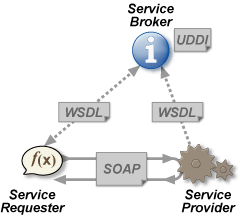
\includegraphics{img/Webservices.png} }}
\end{center}

Wspomniany wcze�niej SOAP, czyli Simple Object Access Protocol, jest form�
elektronicznej koperty, kt�ra zawiera podstawowe informacje o rz�daniu oraz o
odpowiedzi. Jest ona zbudowana w oparciu o j�zyk XML. Drug� kluczow� technologi�
jest j�zyk opisu us�ugi - Web Service Description Language (WSDL). Z jego
pomoc� jeste�my w stanie poinformowa�, jakie us�ugi oferuje nasz serwer oraz
mo�emy wskaza� dok�adny spos�b ich wywo�ywania. W wypadku urz�dze� o
ograniczonej mocy obliczeniowej spotyka si� go tylko przy automatycznym
generowaniu kodu wywo�uj�cego Web Services. Ostatnim fundamentem tej
technologii jest us�uga UDDI (Universal Description, Discovery, and
Integration). Pozwala ona na dynamiczne odnajdowanie innych us�ug Web. 
\newline
Najwi�ksz� wad� tego rozwi�zania jest pewien narzut wydajno�ciowy oraz
pojemno�ciowy, zwi�zany z budow� samych wiadomo�ci. W innych metodach tre��
wiadomo�ci przesy�ana jest w zoptymalizownej postaci kodu binarnego i nie
posiada zwykle �adnych metadanych (co zwykle prowadzi do problem�w z komunikacj�
pomi�dzy r�nymi platformami). W przypadku Web Services, wiadomo�ci przesy�ane
s� w kopercie, zbudowanej na bazie XML, kt�ra posiada du�o nadmiernych
informacji. Powoduje to, �e przy przesy�aniu wiadom�ci ��cze dodatkowo zostaje
obci��one tymi nadmiarowymi danymi. Co wi�cej, po stronie odbiorcy nale�y
przeprowadzi� rozbi�r gramatyczny otrzymanego komunikatu. Zwi�ksza to
zapotrzebowanie na moc obliczeniow�. Mo�e to mie� kluczowe znaczenie w
przypadku urz�dze� mobilnych, kt�re cz�sto dysponuj� bardzo ograniczonymi
zasobami mocy obliczeniowej oraz przepustowo�ci. Szczeg�lnym przypadkiem s�
u�ytkownicy, kt�rzy posiadaj� niezrycza�towany dost�p do sieci i p�ac� r�ne
stawki w zale�no�ci od ilo�ci przes�anych danych. W tym wypadku narzut
pojemno�ciowy Web Services mo�na w spos�b bezpo�redni przeliczy� na koszty,
jakie generuje on dla ca�ej organizacji.
\newline
Z my�l� o bezpiecznej komunikacji przy u�yciu technologii Web Services,
wprowadzono protok� komunikacyjny WS-Security (Web Service Security),
pozwalaj�cy na zaaplikowanie podstawowych standard�w bezpiecze�stwa. Protok�
ten zawiera specyfikacj�, opisuj�c� metody wymuszania integralno�ci oraz
poufno�ci przesy�anych danych. Pozwala na do��czanie do wiadomo�ci SOAP
podpis�w oraz nag��wk�w, zwi�zanych z szyfrowaniem danych. Wspiera tak�e
formaty certyfikacyjne takie jak X.509. Protok� dzia�a w warstwie aplikacyjnej i zosta�
tak zaprojektowany, by zapewni� bezpiecze�stwo od ko�ca do ko�ca (end-to-end
security). Niestety, w obecnej chwili protok� ten nie zosta� zaimplementowany
na urz�dzeniach mobilnych i na pewno w najbli�szym czasie nie stanie si� na
nich standardem. Ograniczeniem s� tu typowe dla tych urz�dze� problemy z
wydajno�ci�. Alternatywnym rozwi�zaniem problemu bezpiecze�stwa jest pos�u�enie
si� zabezpieczeniami na poziomie warstwy transportowej (TLS), takimi jak https.
Pozwala to na zapewnienie bezpiecze�stwa punkt-punkt.
\newline
Technologia Web Services jest godna rozwa�enia przy wyborze sposobu komunikacji
w integracji mobilnej. Istniej� bardzo dobre implementacje, takie jak kSoap,
kt�re dzia�aj� praktycznie na ka�dej platformie wspieraj�cej wirtualn� maszyn�
Java. Pozosta�e platformy, takie jak Blackberry czy WMD (Windows Mobile Device),
r�wnie� posiadaj� stosowne biblioteki, kt�re pozwalaj� w bardzo prosty spos�b
pod��czy� si� do istniej�cej infrastuktury. Znane s� komercyjne rozwi�zania
integracyjne, takie jak Mobile Data Service na platformie Blackberry, kt�re
potrafi� automatycznie generowa� kod, wywo�uj�cy procedury na podstawie podanego
im wcze�niej schematu WSDL. Je�li kluczowym nie jest optymalne wykorzystanie
��cza, czy te� gwarancja dostaczenia, to jest to technologia, kt�rej u�ycie jest
zalecane przy integracji mobilnej, czy te� jakiejkolwiek innej integracji w
�rodowisku Enterprise.

\paragraph{Wiadomo�ci w �rodowisku mobilnym} 
Integracja za pomoc� Web serwis�w
jest do�� prosta do zaimplementowania, stawia jednak przed programist� szereg
problem�w,
kt�re musi on samodzielnie rozwi�za�. Jest to, przede wszystkim, brak gwarancji
dostarczenia komunikatu. Dodatkowo, samodzielnie nale�y obs�u�y� b��dy
transmisji, mo�liwe przerwy i konieczno�� ponownego nawi�zania po��czenia. nie
implikuje to potrzeby uruchamiania brokera wiadomo�ci, kt�ry jest dodatkowym
elementem, zwi�kszaj�cym skomplikowanie systemu. Jednak w sytuacji, gdy w
przedsi�biorstwie dzia�a ju� broker, obs�uguj�cy kilka aplikacji, do��czenie
komponentu mobilnego mo�e by� dobrym rozwi�zaniem. Zastosowanie wiadomo�ci do 
integracji urz�dze� mobilnych niesie ze sob� wszelkie konsekwencje tej metody 
integracji znane z integracji klasycznych system�w informatycznych:

\begin{itemize}
  \item Oddzielenie nadawcy wiadomo�ci od jej odbiorcy. Pozwala to na wysy�anie
  wiadomo�ci nawet wtedy, gdy odbiorca nie jest w stanie jej aktualnie odebra� 
  (na przyk�ad ze wzgl�du na brak po��czenia).
  \item Gwarancja dostarczenia. Z jednej strony, umieszczenie wiadomo�ci w
  kanale komunikacyjnym gwarantuje, �e odbiorca odbierze j� wtedy, gdy b�dzie pobiera� przeznaczone
  dla niego wiadomo�ci. Z drugiej strony, w przypadku niepowodzenia, jest o
  tym fakcie od razu informowany.
  \item Skalowalno��. Wiadomo�ci pozwalaj� na lepsze wykorzystanie
  zasob�w serwer�w. Aplikacje, b�d�ce odbiorcami wiadomo�ci, mog� je odbiera� w
  tempie, w kt�rym s� w stanie je przetwarza�. Wyklucza to wi�c mo�liwo�� ich
  przeci��enia (tutaj oczywistym wymaganiem jest odpowiednio du�a pojemno��
  kolejki wiadomo�ci).
  \item Nadawanie priorytet�w. Dzi�ki wiadomo�ciom, mo�emy przetwarza� ��dania
  zgodnie z ich priorytetem, szczeg�lnie w momentach wysokiego obci��enia.
  Pozwala to na obs�u�enie najpilniejszych wiadomo�ci przed innymi (co nie jest
  mo�liwe bez dodatkowych ingerencji w przypadku Web serwis�w).
  \item Mo�liwo�� stosowania wzorc�w integracyjnych. Droga wiadomo�ci pomi�dzy
  nadawc� i odbiorc� mo�e by� zmieniana w deklaratywny spos�b (pomagaj� tu
  specjalne pakiety integracyjne, np. Apache Camel), co pozwala na dodatkowe
  przetwarzanie, konwertowanie, zmienianie kolejno�ci i inne modyfikacje
  przesy�anych wiadomo�ci. Pod��czenie do kana�u publish-subscribe pozwala na
  �atwe wysy�anie wiadomo�ci do wielu odbiorc�w.
\end{itemize}
Nie jest to, oczywi�cie, technologia pozbawiona wad. To, co musimy wzi�� pod
uwag�, to istnienie wspomnianego ju� brokera wiadomo�ci. Dodatkowo,
wszystkie wspomniane wcze�niej mo�liwo�ci maj� sw�j koszt, jakim jest wi�kszy rozmiar
aplikacji mobilnej, wynikaj�cy z konieczno�ci skorzystania z dodatkowych
komponent�w. Nie jest to du�y narzut w przypadku klasycznych aplikacji.
Zwi�ksza on jednak rozmiary aplikacji mobilnej w stopniu, kt�ry mo�e nie
pozwoli� na jej uruchomienie na prostszych urz�dzeniach.\\
\indent
W przeciwie�stwie do Web serwis�w, nie wykszta�ci� si� jeden, uniwersalny
standard przesy�ania wiadomo�ci. W ramach platformy J2ME naturalnym
rozwi�zaniem jest JMS, pochodz�cy z Javy Enterprise. Jednak inne platformy, jak
Windows Mobile, maj� swoje w�asne rozwi�zania. Warto zwr�ci� uwag� na
fakt, �e stosowanie wiadomo�ci umo�liwia zmian� najni�szej warstwy
komunikacyjnej pomi�dzy urz�dzeniami. O ile w przypadku Web serwis�w oczywistym
wyborem jest po��czenie z internetem, o tyle wiadomo�ci mog� by� przesy�ane
zar�wno w ten spos�b, jak i za pomoc� wiadomo�ci tekstowych. Pozwala to na
funkcjonowanie aplikacji bez utrzymywania sta�ego po��czenia z internetem, co w przypadku
ograniczonej ��czno�ci jest mocno utrudnione. 


% Istnieje kilku dostawc�w
% rozwi�za� opartych o wiadomo�ci z kt�rych najpopularniejsze to IBM MQ Everyplace
% oraz iBus//Mobile.
% \subparagraph{IBM MQ Everyplace}
% \subparagraph{iBus//Mobile}


\indent
Na pytanie, kt�ra metoda, wiadomo�ci czy Web serwisy, jest lepsza, nie ma
jednoznacznej odpowiedzi. Wszystko zale�y od oczekiwa� u�ytkownika, od
integrowanego systemu, jego natury oraz aktualnie istniej�cych komponent�w. Wydaje
si�, �e przed podj�ciem decyzji warto zada� sobie nast�puj�ce pytania: 
\begin{itemize}
  \item Czy potrzebujemy gwarancji dostarczenia komunikatu, czy te� jest to
  system, w kt�rym nie jest to kluczowe? Web serwisy nie zapewniaj� tej
  funkcjonalno�ci i w razie potrzeby musimy j� sami zaimplementowa�.
  \item Czy integrujemy system mobilny z istniej�cymi ju� systemami, kt�re
  porozumiewaj� si� ze sob� za pomoc� brokera wiadomo�ci? W takim wypadku,
  wykorzystanie wiadomo�ci jest naturalnym rozwi�zaniem, pozwalaj�cym na
  dointegrowanie urz�dze� mobilnych do sieci korporacyjnej.
  \item Czy bierzemy pod uwag� znaczne wydatki, kt�re wynikaj� z wykorzystania
  kosztownych, komercyjnych broker�w wiadomo�ci? Wykorzystanie Web serwis�w
  pozwala na znaczne obni�enie koszt�w, wynikaj�cych z obecno�ci wielu
  bezp�atnych platform, opartych na otwartych standardach.
  \item Czy szybki czas dostarczenia jest kluczowy dla dzia�ania naszego
  systemu? Wiadomo�ci wprowadzaj� pewien narzut czasowy, kt�ry jednak nie musi
  by� istotny z naszego punktu widzenia.
\end{itemize}
Po przeanalizowaniu obu metod komunikacji,w cz�ci implementacyjnej naszej
pracy, zdecydowali�my si� na wykorzystanie Web serwis�w z kilku powod�w:
\begin{itemize}
  \item Wykorzystanie komercyjnego oprogramowania nie by�o mo�liwe, a dodatkowo
  wymaga�oby uruchomienia skomplikowanej cz�ci po stronie serwerowej. Naszym
  celem nie by�o konfigurowanie jednej skomplikowanej platformy, ale raczej 
 poznanie problem�w, z kt�rymi nale�y si� liczy�, integruj�c aplikacj�
 mobiln�.
  \item Wykorzystanie powszechnie dost�pnego pakietu kJORAM (bezp�atnej
  implementacji JMS, dost�pnej tak�e dla urz�dze� mobilnych) oznacza�o, tak
  naprawd�, wykorzystanie Web serwis�w, kt�re zosta�y odpowiednio obudowane
  przez tw�rc�w szablonu.
  \item Tworzony przez nas szablon komunikacyjny musia� dzia�a� z jak
  najmniejszym op�nieniem, tak, aby u�ytkownik nie odczuwa� dyskomfortu,
  zwi�zanego z oczekiwaniem na kolejne ekrany. Zastosowanie wiadomo�ci
  wprowadza dodatkowe op�nienie, kt�re nie sprzyja responsywno�ci systemu.
\end{itemize}

  
    
\chapter{Metody realizacji aplikacji mobilnej zorientowanej na �rodowisko
enterprise}

Na wst�pie dyskusji o realizacji mobilnej cz�ci platformy integracyjnej
zwr��my uwag� na dost�pne na rynku urz�dzenia, kt�re posiadaj� preinstalowane
systemy operacyjne pozwalaj�ce na dodawanie nie przewidzianych przez tw�rc�w zewn�trznych
rozwi�za�. Tego typu systemy operacyjne musz� si� charakteryzowa� udost�pnieniem
na zewn�trz, do instalowanych przez nas aplikacji, pewnego API pozwalaj�cego na
realizacj� podstawowych us�ug, takich jak transfer danych czy ich sk�adowanie w
pami�ci urz�dzenia. Na chwile obecn� (pierwszy kwarta� 2009 roku) na rynku
dost�pne s� urz�dzenia dzia�aj�ce w oparciu wymienione poni�ej platformy mobilne :
\begin{itemize} 
\item{WMD - Windows Media Devices oparte o system operacyjny Windows Mobile
opracowany przez firm� Microsoft}
\item{Symbian - platforma spotykana g��wnie na
smartfonach oferowanych przez firmy takie jak Nokia czy Samsung}
\item{Blackberry - marka wypromowana prze firm� Research in Motion, oferuje
urz�dzenia z preistalowanym systemem operacyjnym opartym na wirtualnej maszynie Java}
\item{Android - system operacyjny oparty na Linuxie, mo�liwy do rozbudowywania
g��wnie przez aplikacje J2ME (w obecnej chwili system jest w fazie test�w) }
\item{pozosta�e autorskie systemy operacyjne, udost�pniaj�ce standardow�
maszyn� wirtualn� Java}
\end{itemize}

Po dok�adnym przyjrzeniu si� powy�szym platformom nasuwa si� jeden stanowczy
wniosek - poza platformami opartymi na J2ME, wykonanie jednej, sp�jnej
aplikacji spe�niaj�cej za�o�enia interoperacyjno�ci jest praktycznie niemo�liwe. Jedynym
rozwi�zaniem jest przygotowanie kilku instancji tej samej aplikacji, kt�re
niestety nie b�d� mia�y ze sob� niczego wsp�lnego poza przyj�tymi za�o�eniami
dotycz�cymi podstawowej funkcjonalno�ci. Wynika to mi�dzy innymi z tego, �e
ka�da platforma oferuje inne mo�liwo�ci i przy okazji wprowadza inne ograniczenia. Co wi�cej tego
typu r�nicowanie wyst�puje r�wnie� w obr�bie samych platform. Na przyk�ad J2ME
posiada profile zwi�zane na sta�e z modelami urz�dze�, kt�re decyduj� o tym,
jakie funkcjonalno�ci dost�pne s� dla program�w. Wskazane powy�ej ograniczenia
techniczne wymuszaj� przy pr�bie wej�cia na rynek aplikacji mobilnych, ju� na
etapie planowania produktu, wybranie konkretnej platformy docelowej, na jakiej
oferowane b�dzie nasze rozwi�zanie. Wraz z sukcesem rozwi�zania, mo�liwa b�dzie
dalsza ekspansja na pozosta�e platformy. Przed t� ostateczn� ewaluacj� warto�ci
pomys�u na produkt, jest bardzo ryzykownym podj�cie pr�by r�wnoleg�ego
wprowadzenia go na r�nych, niekompatybilnych platformach. Zwi�ksza to znacznie
pr�g wej�cia oraz utrudnia poprawn� kontrol� nad stopniem dojrza�o�ci produktu.
Co wi�cej przy s�abym zarz�dzaniu funkcjonalno�ciami mo�e wyst�pi� problem
powstania r�nic funkcjonalnych pomi�dzy r�nymi wersjami naszej aplikacji. Tego
typu problemy wp�yn� w spos�b bezpo�redni na postrzeganie naszego produktu przez klient�w, w
szczeg�lno�ci gdy b�dziemy mieli do czynienia z korporacjami, w obr�bie kt�rych
stosowane s� r�ne rozwi�zania mobilne. 
\newline
Uzbrojeni w wiedz� o pewnych mo�liwych do napotkania problemach skupimy teraz
nasz� uwag� na doborze metodologii, wed�ug kt�rej b�dzie powstawa�a nasza
aplikacja. Wyboru dokonuje si� zwykle spo�r�d trzech klasycznych podej��. S�
to:

\begin{itemize}
  \item Budowa aplikacji w oparciu o przegl�dark� mobiln�
  \item Budowa aplikacji przy u�yciu generatora aplikacji
  \item Budowa aplikacji od podstaw (przy ewentualnym wsparciu
  szkielet�w aplikacyjnych)
\end{itemize}

Ka�de z tych podej�� ma swoje wady i zalety, kt�re powoduj�, �e mo�na do nich
przypisa� r�ne zastosowania. W nast�pnych rozdzia�ach przyjrzymy si� ka�demu z
tych podej�� wyr�niaj�c najwa�niejsze cechy ka�dego z nich oraz przedstawiaj�c
pewne nieroz��cznie zwi�zane z nimi �rodowiska uruchomieniowe oraz
programistyczne.
 
\section{Przegl�darka mobilna}

Urz�dzenia mobilne, w tym telefony kom�rkowe, maj� wbudowane przegl�darki
internetowe, za pomoc� kt�rych coraz cz�ciej mo�na przegl�da� wszystkie
dost�pne w Internecie strony (w przeciwie�stwie do sytuacji sprzed kilku lat,
gdy jedynie cz�� z nich, posiadaj�ca wersj� WAP, by�a dost�pna). W przeci�gu
bardzo kr�tkiego czasu dokona� si� du�y post�p w rozwoju mobilnych
przegl�darek. Ci�gle jednak nie zapewniaj� one wygody por�wnywalnej z
przegl�daniem stron na tradycyjnym komputerze. Jednak�e korzystanie z
aplikacji, zbudowanych w oparciu o model tr�jwarstwowy (z u�yciem tak zwanego 
cienkiego klienta - czyli przegl�darki WWW), niesie za sob� szereg korzy�ci,
takich jak brak potrzeby instalowania aplikacji, �atwo�� wdro�enia czy wreszcie du�a
przeno�no�� pomi�dzy r�nymi platformami.

\subsection{Rodzaje przegl�darek mobilnych}

Omawiaj�c temat przegl�darek mobilnych nale�y zwr�ci� uwag� na to, �e na rynku
znajduje si� obecnie wiele tego typu produkt�w. Nie wszystkie s� bezpo�redni�
konkurencj�. Cz�� z nich mo�e dzia�a� tylko w obr�bie platformy, na kt�r�
zosta�y zaprojektowane. Szczeg�lnie widoczne jest to w wypadku przegl�darki
Safari, kt�ra jest u�ywa praktycznie tylko na urz�dzeniach mobilnych firmy
Apple. Nale�y bra� to pod uwag� przy projektowaniu strony mobilnej. Mo�e
si� okaza�, �e mo�na ograniczy� wysi�ki zapewnienia pe�nej zgodno�ci na
wszystkich mo�liwych przegl�darkach, poniewa� w obr�bie organizacji funkcjonuj�
urz�dzenia tylko jednej marki (na przyk�ad Blackberry).


\subsubsection{Uproszczone przegl�darki mobilne}

Pierwszym rodzajem przegl�darek, spotykanych na urz�dzeniach mobilnych, s�
przegl�darki, wy�wietlaj�ce uproszczon� wersj� stron internetowych.
W zwi�zku z tym, przeniesienie istniej�cych portali korporacyjnych pod
platform�, kt�ra ich u�ywa, wi��e si� z dodatkow� prac�, wynikaj�c� z
konieczno�ci przystosowania sposobu wy�wietlania portali do mo�liwo�ci przegl�darki.

\index{Opera Mini}
\paragraph{Opera Mini}

\begin{figure}[htb]
    \begin{center}
    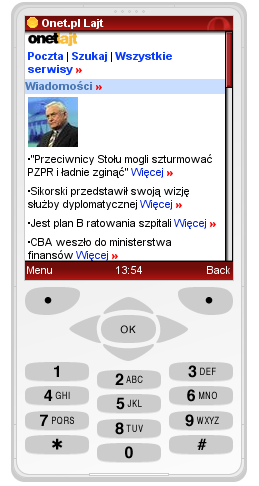
\includegraphics[angle=0,scale=0.6]{img/opera_onet.png}
    \end{center}
    \caption{Przyk�adowa strona wy�wietlona w przegl�darce Opera Mini}
    \label{fig:ominionet}
\end{figure} 

Jest to najpopularniejsza przegl�darka mobilna, dzia�aj�ca w oparciu o platform�
Java 2 Micro Edition. Charakterystyczn� cech� tej przegl�darki jest serwer
proxy, kt�ry optymalizuje zawarto�� stron przed za�adowaniem. Wad� tego
rozwi�zania mo�e by� niech�� do u�ywania go w przedsi�biorstwach przy pr�bie
uzyskania dost�pu do wra�liwych danych. Strach przed ich kradzie�� mo�e by� du�o
wi�kszy ni� korzy�ci, jakie mo�na odnie�� z u�ywania tego programu.



\index{Blackberry}
\paragraph{Blackberry Browser}

\begin{figure}[htb]
    \begin{center}
    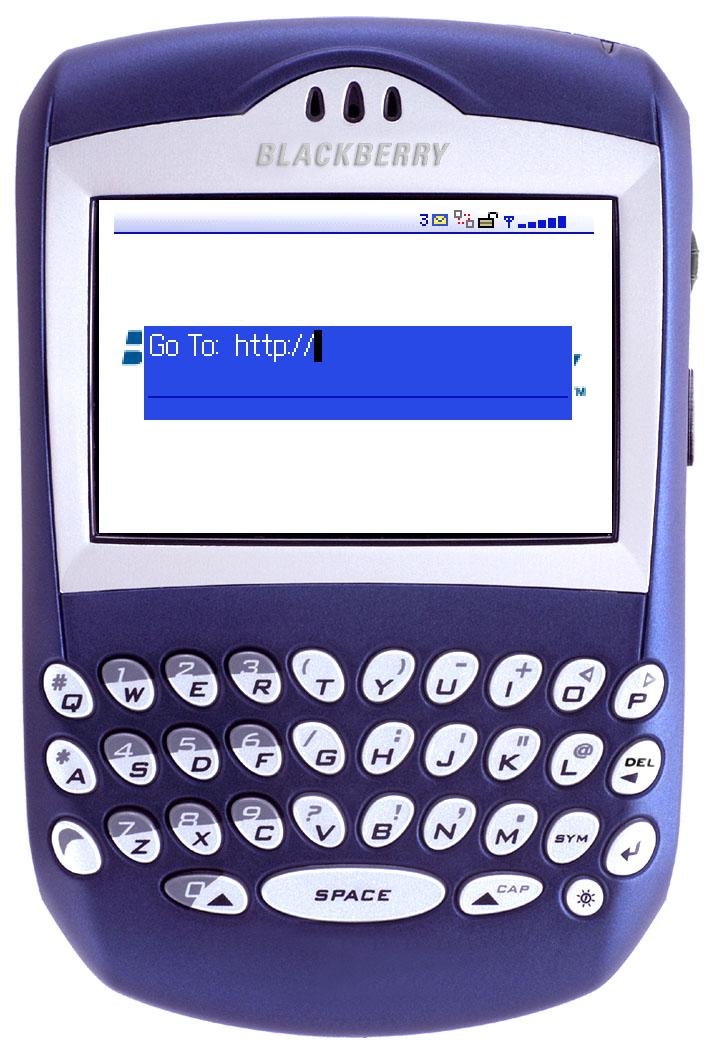
\includegraphics[angle=0,scale=0.2]{img/7290.jpg}
    \end{center}
    \caption{Przyk�adowa strona wy�wietlona w przegl�darce BlackBerry}
    \label{fig:blackberrybrowser}
\end{figure}  

Blackberry Browser jest domy�ln� aplikacj�, pozwalaj�c� na przegl�danie zasob�w
intranetu lub internetu. Podstawowym trybem dzia�ania tej przegl�darki jest
umo�liwianie dost�pu do wewn�trznych zasob�w firmy. Wi��e si� to bezpo�rednio
ze sposobem dzia�ania urz�dze� Blackberry, opartym o sie� wirtualn�. Ka�de
urz�dzenie mobilne jest tunelowane przez powszechnie dost�pn� sie�
telekomunikacyjn� do sieci wewn�trznej firmy. Tunelowaniem zajmuje si�
dzia�aj�cy w obr�bie firmowej sieci serwer BES (Blackberry Enterprise Server).
Jest on jedynym elementem wystawionym na zewn�trz i, poprzez szyfrowane
po��czenie, umo�liwia przekierowywanie pakiet�w z i do urz�dze� mobilnych.
Dzi�ki temu, ka�dy u�ytkownik ma zapewniony bezpieczny dost�p do informacji
firmowych. Ma to ogromne znaczenie przy wyborze sposobu umobilniania. W
przypadku pozosta�ych przegl�darek mobilnych, jedyn� gwarancj� bezpiecze�stwa
jest https, przy czym nie ma �adnego zapewnienia bezpiecze�stwa danych, kt�re
przechodz� przez serwery proxy (tak, jak w wypadku przegl�darki Opera Mini).
Tak wi�c w wypadku, gdy g��wnym czynnikiem dycyduj�cym o wyborze jest
bezpiecze�stwo, warto rozwa�y� zastosowanie rozwi�za�, kt�re je gwarantuj�.





\subsubsection{Pe�ne przegl�darki mobilne}
\index{Opera Mobile}
\paragraph{Opera Mobile}


\begin{figure}[htb]
    \begin{center}
    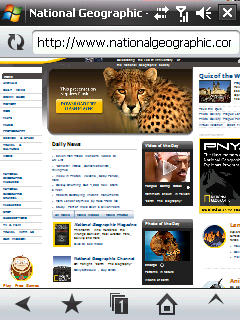
\includegraphics[angle=0,scale=0.8]{img/opera_mobile.png}
    \end{center}
    \caption{Przyk�adowa strona wy�wietlona w przegl�darce Opera}
    \label{fig:operabrowser}
\end{figure}  


Opera Mobile jest jedn� z najpopularniejszych pe�nowarto�ciowych
przegl�darek mobilnych. Zosta�a zbudowana na bazie silnika przegl�darki
stacjonarnej. Zachowuje prawie ca�kowit� zgodno�� z pe�n� wersj�, co oznacza, �e
w �rodowisku opartym tylko i wy��cznie o t� mark�, mo�liwe jest u�ywanie stron
internetowych bez �adnych zmian, przystosowuj�cych je do wersji mobilnej.
Niestety, ze wzgl�du na niewielk� popularno�� przegl�darki stacjonarnej oraz jej
ca�kowity brak zgodno�ci z dwoma dominuj�cymi przegl�darkami (wynikaj�cy z
bardzo restrykcyjnego pilnowania standard�w przez deweloper�w Opery), zwykle
niezb�dne s� zmiany w konstrukcji strony. Dzia�a na urz�dzeniach korzystaj�cych
z platform Symbian S60 oraz Windows Mobile.

\index{Internet Explorer Mobile}
\paragraph{Internet Explorer Mobile}


\begin{figure}[htb]
    \begin{center}
    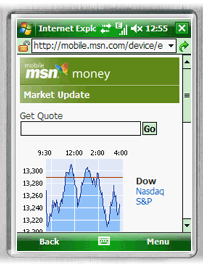
\includegraphics[angle=0,scale=0.8]{img/ie_mobile.png}
    \end{center}
    \caption{Przyk�adowa strona wy�wietlona w przegl�darce Internet Explorer
    Mobile}
    \label{fig:iebrowser}
\end{figure}  


W zwi�zku z tym, �e firma Microsoft posiada od dawna systemy operacyjne
przeznaczone na platformy mobilne (Windows Mobile oraz starszy Windows CE) razem z nimi zawsze
dostarczana jest przegl�darka internetowa. Jest sporo wolniejsza od
konkurencji, ale ze wzgl�du na fakt, �e jest preinstalowana na platformach,
cieszy si� du�ym powodzeniem w�r�d mobilnych u�ytkownik�w. Przy wdra�aniu
rozwi�za� mobilnych w firmie, w kt�rej u�ywane s� urz�dzenia typu Pocket PC,
nale�y si� spodziewa�, �e zostanie ona narzucona z g�ry jako klient naszej
mobilnej strony internetowej. Pozwala na dzia�anie zar�wno w trybie mobilnym,
odczytuj�cym uproszczony zapis html, jak i na prac� z pe�nymi wersjami stron
internetowych. Niestety, silnik tej przegl�darki zosta� napisany zupe�nie od
nowa, przez co nie jest w pe�ni zgodny z tym, kt�ry jest u�ywany w pe�nej wersji
przegl�darki Internet Explorer. Mo�e to zwi�kszy� nak�ad pracy niezb�dny do
uzyskania mobilnej wersji naszej strony. 


\index{Safari}
\paragraph{Safari}

\begin{figure}[htb]
    \begin{center}
    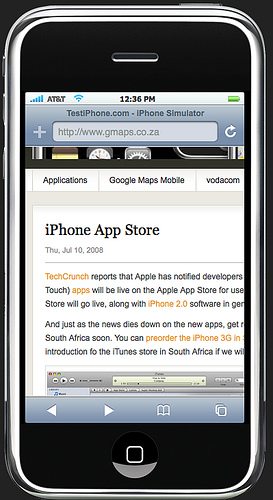
\includegraphics[angle=0,scale=0.4]{img/iphone_screen.jpg}
    \end{center}
    \caption{Przyk�adowa strona wy�wietlona w przegl�darce Safari
    Mobile}
    \label{fig:safaribrowser}
\end{figure}  

Przegl�darka firmy Apple u�ywana jest g��wnie w jej produktach. Jej mobilna
wersja pojawi�a si� na rynku w momencie wprowadzenia telefonu iPhone.
Charakteryzuje si� bardzo dobr� obs�ug� j�zyka JavaScript oraz pe�n� zgodno�ci�
z jej wersj� stacjonarn�. W odr�nieniu od produkt�w Opera Software na
urz�dzeniach stacjonarnych firmy Apple, jest ona przegl�dark� dominuj�c�, wi�c
dzi�ki pe�nej zgodno�ci, nak�ady pracy potrzebne na przystosowanie oraz
wdro�enie s� znacznie mniejsze ni� w przypadku konkurencji.



\index{projektowanie stron}
\subsection{Zagadnienia zwi�zane z projektowaniem stron}

W poprzednich rozdzia�ach zosta�o przedstawionych kilka najpopularniejszych
przegl�darke mobilnych. Wyr�nione zosta�y pewne elementy, kt�re wymuszaj�
zastosowanie specjalnej metodologii przy przystosowywaniu stron internetowych.
Podzia� na przegl�darki uproszczone i pe�ne przegl�darki mobilne sugeruje dwa
r�ne podej�cia do tego zagadnienia. Pierwszy spos�b przystosowania stron
internetowych zak�ada, �e mamy do czynienia z pe�nymi przegl�darkami. W zwi�zku
z tym, �e r�ni� si� one g��wnie brakiem wsparcia dla niekt�rych element�w
j�zyka Javascript, to praca, zwi�zana z ich umobilnianiem, wi��e si� g��wnie z
upraszczeniem pewnych element�w lub przepisywaniem ich tak, by by�y
kompatybilne. Zwykle trzeba zrezygnowa� te� z pewnych zaawansowanych
funkcjonalno�ci, kt�re dzia�aj� w oparciu o technologi� j�zyka Javascript. Je�li
projektujemy portal od pocz�tku, to mo�emy w bardzo prosty spos�b,
przestrzegaj�c kilku podstawowych regu�, umo�liwi� dost�p do niego z urz�dze�
mobilnych. Najwa�niejsze aspekty, kt�re nale�y mie� na uwadze to:
\begin{itemize}
  \item Nale�y pami�ta� o budowaniu prostych i funkcjonalnych uk�ad�w stron.
  Dotyczy to w szczeg�lno�ci form, kt�re powinny mie�ci� si� na jednym ekranie.
  Co wi�cej, nale�y wykorzystywa� listy opcji tam, gdzie tylko si� da, tak, by
  u�ytkownik musia� w minimalnym stopniu u�ywa� klawiatury.
  \item Nie mo�na zak�ada�, �e do nawigacji b�dzie wykorzystywana wirtualna
  myszka. Nale�y tak projektowa� strony, by mo�na by�o je obs�ugiwa� innymi
  rodzajami kontroler�w (na przyk�ad przy pomocy technologii trackwheel).
  Wprowadzanie danych z klawiatury urz�dzenia mobilnego jest bardzo niewygodne,
  wi�c nale�y zadba� o to, by u�ytkownik nie musia� wprowadza� du�ych ilo�ci
  danych(wspomniane wcze�niej listy opcji rozwi�zauj� w pewnym stopniu ten
  probem)
  \item Urz�dzenia mobilne dysponuj� innymi, cz�sto znacznie mniejszymi
  rozdzielczo�ciami ni� systemy stacjonarne. Niekt�re przegl�darki, takie jak
  Opera Mobile, oferuj� funkcje szybkiej nawigacji w obr�bie du�ych stron,
  dzi�ki czemu problem ten jest w pewien spos�b ograniczany. Je�li jednak chcemy
  dostarczy� nalepsz� mo�liw� obs�ug� stron, to nale�y wykorzysta� pewne
  elementy CSS, takie jak zapytania o typ urz�dzenia, aby dostosowa� stron� do
  konkretnej rozdzielczo�ci. Dobrym przyk�adem, jak wa�ne jest uwzgl�dnienie
  tych rozbie�no��i, jest Opera Desktop oraz Opera Mini. Na rysunku
  \ref{fig:omini} wida� przyk�adow� realizacj� strony z wykorzystaniem specjalnych styl�w dla
  przegl�darki moblinej.
  \begin{figure}[htb]
    \begin{center}
    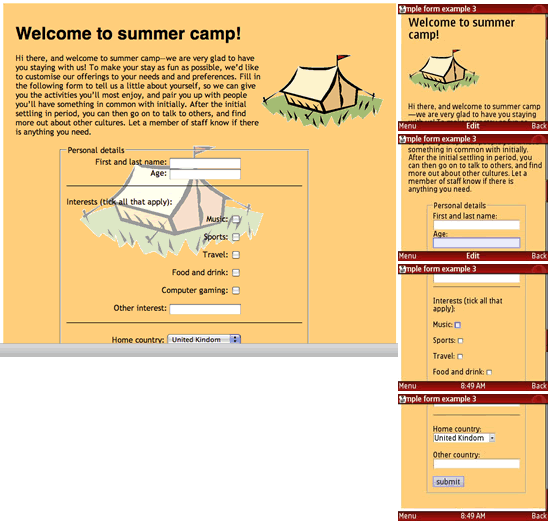
\includegraphics[angle=0,scale=.6]{img/desktopmobile.png}
    \end{center}
    \caption{Ta sama strona otwarta w Opera Desktop 9.5 oraz Opera Mini 4.1}
    \label{fig:omini}
\end{figure} 

  \item  Nale�y r�wnie� wzi�� pod uwage r�nice pomi�dzy przegl�darkami
 mobilnymi - w szczeg�lno�ci oferowanymi przez r�nych producent�w. R�nice w
 silnikach tych przegl�darek bywaj� tak du�e, �e cz�sto projektant jest
 zmuszony do przygotowywania r�nych wersji tej samej strony dla r�nych
 urz�dze� mobilnych. Niezgodno�ci te wynikaj� g��wnie z nieprzestrzegania
 standard�w przez producent�w oraz z wprowadzania do swoich rozwi�za�
 dodatkowych funkcjonalno�ci, niespotykanych na innych platformach. Dobrym
 przyk�adem takich dzia�a� jest wprowadzenie w najnowszej wersji mobilnej
 przegl�darki Safari na urz�dzeniu iPhone mo�liwo�ci budowaniu animacji
 poklatkowych przy pomocy samych styl�w CSS. Jest to bardzo ciekawa i przydatna
 funkcjonalno��, ale ca�kowicie nie przeno�na na inne przegl�darki.

\end{itemize}
 
\section{Generatory aplikacji}
\index{Generatory aplikacji}
Wielu producent�w podejmuje pr�by zbudowania �rodowisk, umo�liwiaj�cych szybkie
tworzenie aplikacji mobilnych (tak zwane RAD - Rapid Application Development).
Maj� one ��czy� zalety obu przedstawionych wcze�niej �wiat�w :

\begin{itemize} 
\item{Pozwala� na �atwe i~szybkie tworzenie aplikacji dost�powych - tak jak
mobilne przegl�darki}
\item{Dostarcza� elastyczno�ci i~rozbudowanych interfejs�w u�ytkownika - tak
jak aplikacje mobilne}
\end{itemize}

W dalszej cz�ci niniejszej pracy przedstawione zostan� dwa tego typu
rozwi�zania, pozwalaj�ce na oszcz�dzenie znacznej ilo�ci pracy przy budowaniu
nowych aplikacji.

\index{Blackberry}
\subsubsection{Generator dedykowany - Blackberry MDS}
\index{Blackberry MDS}
Blackberry MDS jest przyk�adem narz�dzia wyspecjalizowanego do tworzenia
aplikacji tylko i~wy��cznie na platform� jednego producenta. Rozwi�zanie to
opiera si� na integracji ma�ej aplikacji zainstalowanej na urz�dzeniach
klienckich (MDS Runtime) z us�ug� typu Web Service dzia�aj�c� na serwerze. 
Dzi�ki niemu mo�liwe jest tworzenie aplikacji, u�ywaj�c podej�cia opisowego.
Zamiast pisa� ca�� aplikacj�, u�ywaj�c j�zyka programowania wraz z
bibliotekami, oferuj�cymi interfejs u�ytkownika, mo�emy przy u�yciu graficznego
edytora projektowa� takie elementy, jak ekrany czy pola z danymi. Wszystko to
przy u�yciu standardowego drag and drop. Nast�pnie, mo�emy po��czy� tak
zbudowane komponenty przy u�yciu r�nych przewodnik�w(wizards), czy te�
edytor�w. Co wi�cej, aplikacja MDS daje nam pe�n� kontrol� nad przep�ywem
sterowania - przy pomocy j�zyka JavaScript jeste�my w stanie zaimplementowa� niemal dowoln�
logik� aplikacji. Aplikacje typu enterprise oraz �r�d�a danych dost�pne s� dla
aplikacji mobilnej poprzez standardow� technologi� Web Services.

\begin{figure}[htb]
    \begin{center}
    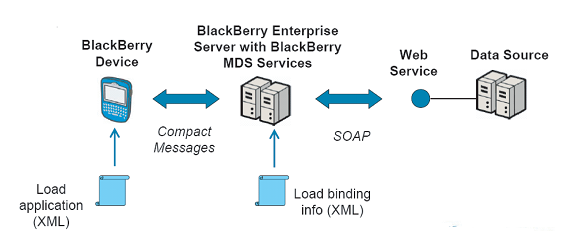
\includegraphics[angle=0,scale=0.7]{img/mds1.png}
    \end{center}
    \caption{Architektura aplikacji opartej o BlackBerry MDS}
    \label{fig:mds1}
\end{figure} 

\index{BES}
\index{Blackberry Enterprise Server}

Aplikacja MDS dla Blackberry jest to aplikacja typu rich-client, zbudowana na
podstawie metadanych zdefiniowanych w j�zyku XML. Te metadane wraz z zasobami,
takimi jak obrazki, gromadzone s� w pakietach, kt�re nast�pnie publikowane s� na
serwerze BES. Serwer ten przy u�yciu technologii push rozsy�a aplikacje do
terminali mobilnych Blackberry. Dzi�ki scentralizowanej metodzie
dystrybucji oraz zarz�dzania aplikacjami mobilnymi, koszty utrzymania mobilnej
infrastruktury s� znacznie ni�sze.

\begin{figure}[htb]
    \begin{center}
    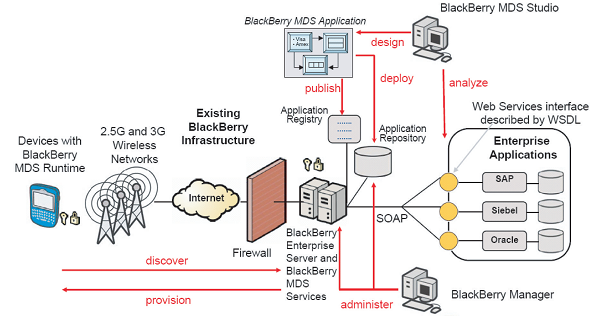
\includegraphics[angle=0,scale=0.7]{img/mds2.png}
    \end{center}
    \caption{Spos�b zarz�dzania aplikacjami opartymi o MDS}
    \label{fig:mds2}
\end{figure} 


\paragraph{Us�uga Blackberry MDS}
Us�uga MDS Blackberry zosta�a zaprojektowana tak, by umo�liwi� wymian� danych
pomi�dzy urz�dzeniami Blackberry, a aplikacjami typu enterprise. Zapewnia ona:
\begin{itemize} 
\item{Izolacj� platformy od szczeg��w, zwi�zanych z integracj� �r�de� danych}
\item{Standard asynchronicznej wymiany komunikat�w}
\item{Przezroczyste dla u�ytkownika i~developera protoko�y bezpiecze�stwa}
\item {Transformacje wiadomo�ci}
\item {Wspomnian� wcze�niej scentralizowan� administracj� przy pomocy
technologii push}
\end{itemize}

\paragraph{Blackberry MDS runtime}
\index{MDS runtime}
Po stronie urz�dzenia mobilnego zainstalowany jest kontener aplikacji MDS.
Zajmuje si� on instalacj�, wyszukiwaniem oraz przegl�daniem aplikacji MDS.
Dostarcza r�wnie� niezb�dne funkcjonalno�ci do tych aplikacji, takie jak
interfejs u�ytkownika, kontener danych oraz us�ugi komunikacyjne klient-serwer.
\index{Netbeans}
\subsubsection{Generator uniwersalny - Netbeans Mobile IDE}

Drugim przyk�adem generatora aplikacji mobilnych jest Netbeans Mobility Pack
oraz zwi�zane z nim �rodowisko programistyczne Netbeans. W przeciwie�stwie do
poprzedniego przyk�adu, to �rodowisko pozwala budowa� uniwersalne aplikacje,
kt�re dzia�aj� na niemal�e dowolnej platformie mobilnej wspieraj�cej J2ME.
Rozpoczynaj�c tworzenie aplikacji powinni�my zwr�ci� uwag� ba udogodnienia
przygotowane przez tw�rc�w Netbeans. Zamiast pisa� setki linijek kodu Java,
mo�emy u�y� specjalnych narz�dzi generuj�cych go dla nas. Do konfigurowania
preferowanego przez nas zachowania aplikacji s�u�� interaktywne diagramy
przep�ywu sterowania pomi�dzy ekranami aplikacji oraz graficzne edytory
interfejsu u�ytkownika, pozwalaj�ce na budowanie z gotowych komponent�w
ekran�w naszej mobilnej aplikacji. Poni�ej przedstawiony jest przyk�ad diagramu
przep�ywu sterowania aplikacji typu Hello World.


\begin{figure}[htb]
    \begin{center}
    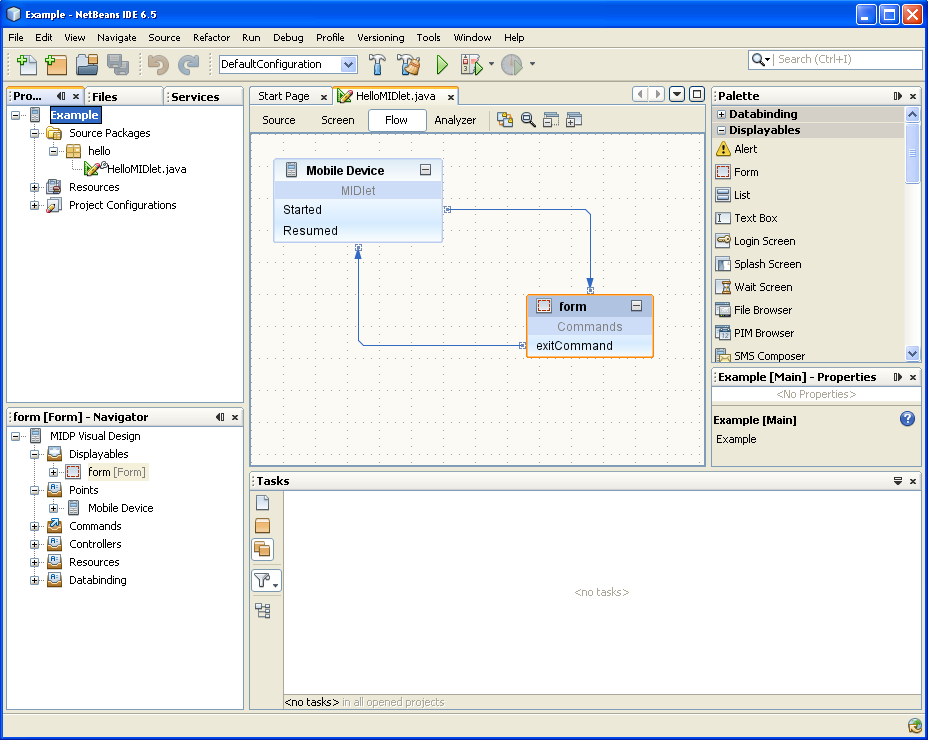
\includegraphics[angle=0,scale=0.4]{img/netbeans_layout.png}
    \end{center}
    \caption{�rodowisko NetBeans z diagramem przep�ywu}
    \label{fig:netbeans_layout}
\end{figure} 


Przyk�adowy diagram przep�ywu sk�ada si� z dw�ch element�w - bloku,
reprezentuj�cego stan wyj�ciowy aplikacji mobilnej (a jednocze�nie stan ko�cowy)
oraz bloku, reprezentuj�cego g��wny i~jedyny ekran. Elementy te po��czone s�
dwiema strza�kami, kt�re przedstawiaj� przep�yw sterowania. Strza�ka skierowna w
stron� formy ma sw�j pocz�tek w zdarzeniu Started. Jest to zdarzenie wywo�ywane
w momencie uruchomienia aplikacji. Dzi�ki takiej konfiguracji, natychmiast po
inicjalizacji aplikacja przechodzi do ekranu g��wnego. Strza�ka w drug� stron�
podpi�ta jest do komendy exitCommand. Wyzwala ona zamkni�cie aplikacji (jej
drugi koniec wskazuje blok wyj�ciowy).
Ekran g��wny zosta� zaprojektowany tak, by wy�wietli� napis oraz komend�,
pozwalajac� na opuszczenie aplikacji.

\begin{figure}[htb]
    \begin{center}
    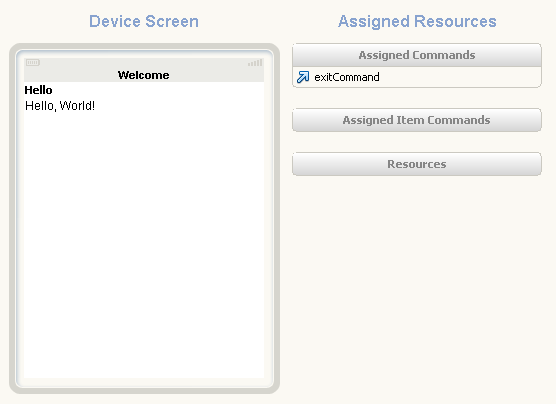
\includegraphics[angle=0,scale=0.5]{img/netbeans_design.png}
    \end{center}
    \caption{Tworzenie interfejsu u�ytkownika w �rodowisku NetBeans}
    \label{fig:netbeans_design}
\end{figure} 



Tak jak wspomniano wcze�niej, tego typu ekrany buduje si� z gotowych
komponent�w. �rodowisko Netbeans udost�pnia zestaw predefiniowanych komponent�w
o podstawowej funkcjonalno�ci. U�ytkownik mo�e odnale�� je na palecie bocznej
programu. W wersji 6.5 paleta ta wygl�da tak, jak na poni�szym rysunku.

\begin{figure}[htb]
    \begin{center}
    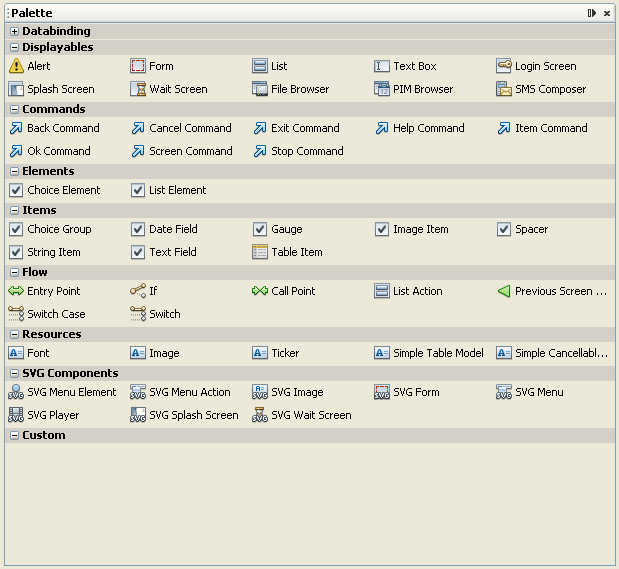
\includegraphics[angle=0,scale=0.5]{img/netbeans_palette.png}
    \end{center}
    \caption{Paleta komponent�w w �rodowisku NetBeans}
    \label{fig:netbeans_palette}
\end{figure} 


Komponentowe budowanie aplikacji znacznie przyspiesza proces ich tworzenia. Co
wi�cej, w razie potrzeby istnieje mo�liwo�� definiowania w�asnych komponent�w,
kt�re p�niej mo�na wykorzystywa� w wielu aplikacjach mobilnych. Miejsce na
w�asne komponenty mo�na zobaczy� w zak�adce custom na standardowej palecie
komponent�w.
Dzi�ki zastosowaniu przedstawionych wcze�niej edytor�w, uda�o si� zbudowa�
bardzo prost� aplikacj� zdoln� do wy�wietlenia napisu. Zosta�o to zrobione bez
napisania linijki kodu w j�zyku Java, u�ywaj�c jedynie narz�dzi graficznych.
Tak zbudowana aplikacja dzia�a na praktycznie ka�dej konfiguracji mobilnej i
gwarantuje jednakowe zachowanie pomi�dzy r�nymi platformami. 

\begin{figure}[htb]
    \begin{center}
    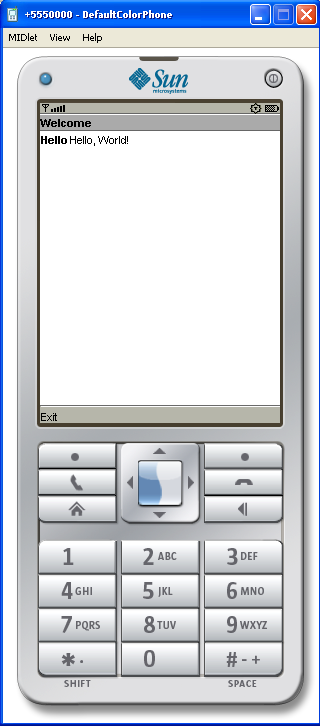
\includegraphics[angle=0,scale=0.5]{img/netbeans_simulator.png}
    \end{center}
    \caption{Emulator telefonu dostarczany przez Suna}
    \label{fig:netbeans_simulator}
\end{figure}

Do konstruowania bardziej zaawansowanych aplikacji nale�y pos�u�y� si�
j�zykiem Java. Dost�p do kodu �r�d�owego automatycznie generowanej aplikacji
pozwala na elastyczne modyfikowanie jej zachowania w zakresie du�o szerszym ni� pozwala na
to jakakolwiek graficzna konfiguracja. Co wi�cej, ka�dy element, kt�ry zosta�
przez nas skonfigurowany w jednym ze wspomnianych wcze�niej edytor�w jest
powi�zany z wygenerowanym kodem w j�zyku Java, z kt�rym mo�na si� zapozna� w
zak�adce source.

\begin{figure}[htb]
    \begin{center}
    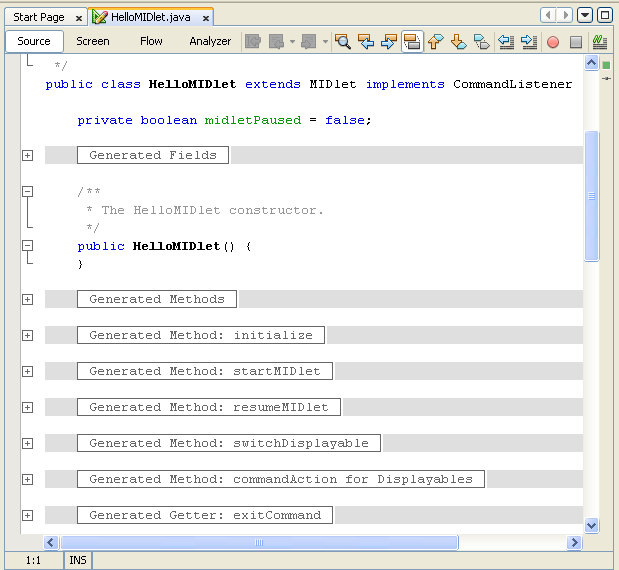
\includegraphics[angle=0,scale=0.5]{img/netbeans_source.png}
    \end{center}
    \caption{Edycja kodu �r�d�owego w NetBeans}
    \label{fig:netbeans_source}
\end{figure}


Wyszarzone obszary to kod, kt�ry zosta� automatycznie wygenerowany przez
�rodowisko Netbeans. W pozosta�ych obszarach mo�na wprowadza� w�asny kod w
j�zyku Java, kt�ry mo�e kontrolowa� dowolne aspekty zachowania si� aplikacji
mobilnej.

Przedstawione �rodowisko programistyczne jest jednym z popularniejszych podej��
do problemu szybkiego konstruowania aplikacji mobilnych. Jest elastyczne i
efektywne, dlatego pos�u�ymy si� nim przy budowie przyk�adowego systemu. 
 
\section{Rozwi�zania dedykowane}

Innym podej�ciem, przypominaj�cym aplikacje zbudowane w oparciu o model
dwuwarstwowy, jest stworzenie aplikacji mobilnej, kt�ra samodzielnie ��czy si�
z Internetem i umo�liwia wy�wietlanie i modyfikacj� danych w spos�b
przewidziany przez jej tw�rc�w. Ogranicza to oczywi�cie funkcjonalno�� takiej
aplikacji do zakresu przewidzianego w danej wersji, a wszelkie zmiany wymagaj�
jej aktualizacji. W zamian za to otrzymujemy wi�ksz� szybko�� dzia�ania,
mo�liwo�� walidacji danych po stronie klienta oraz elastyczno�� w tworzeniu
interfejsu (kt�ry w tym przypadku nie jest ograniczony do kontrolek
zapewnianych przez przegl�dark� WWW).

Wad�, z kt�rej niewiele os�b zdaje sobie
spraw�, jest mniejsza przeno�no�� aplikacji, cho�by by�y one napisane w j�zyku
projektowanym z my�l� o niezale�no�ci od platformy, takim jak Java. Wynika ona
z r�norodno�ci urz�dze� dost�pnych na rynku. Ca�kowita przeno�no�� mo�liwa
jest do uzyskania tylko dla prostych aplikacji, nie korzystaj�cych z
mo�liwo�ci oferowanych przez konkretne modele urz�dze� mobilnych. Przy pr�bie
zbudowania czegokolwiek wi�kszego natychmiast natkniemy si� na niewidzialny mur
generowany przez ogromne r�nice pomi�dzy dost�pno�ci� profili na
poszczeg�lnych platformach oraz przez r�nice w implementacji pewnych cz�ci
samych maszyn wirtualnych. Co wi�cej tu opisana sytuacja wskazuje na problem,
kt�ry generuje stworzona z my�la o przeno�no�ci platforma J2ME. Jeszcze wi�ksze
problemy pojawiaj� si� gdy chcemy rozszerzy� zasi�g naszej aplikacji o kolejne
segmenty rynku, takie jak u�ytkownicy system�w Symbian czy Windows Mobile. W
tym momencie okazuje si�, �e zostaniemy zmuszeni do napisania nie jednej
aplikacji, ale wielu, kt�re cz�sto mog� nie mie� prawie �adnych cz�ci
wsp�lnych. 

\chapter{Szablon komunikacyjny}

Do zademonstrowania mo�liwo�ci komunikacyjnych pomi�dzy systemem stacjonarnym i
mobilnym stworzyli�my szablon u�atwiaj�cy tworzenie aplikacji posiadaj�cych
mobilny interfejs, z poziomu kt�rego mo�na sterowa� aplikacj� serwerow�.
Rozwi�zanie, kt�re przyj�li�my jest na tyle og�lne, �e umo�liwia rozwi�zanie
kilku podobnych problem�w, kt�re przedstawimy dalej.
\newline
Ide� stoj�c� za stworzeniem szablonu by�o po��czenie zalet zapewnianych przez
aplikacj� zbudowan� w oparciu o model tr�jwarstwowy z tymi typowymi
dla samodzielnej aplikacji. Stworzone rozwi�zanie stanowi raczej pomys�, kt�ry
mo�na rozwija� i wykorzystywa� do budowy bardziej skomplikowanych system�w.
Dlatego te� mo�liwo�ci takiego podej�cia nie s� ograniczone przez stworzony
szablon.
\newline
Szablon sk�ada si� z dw�ch cz�ci - mobilnej i serwerowej.
U�ytkownik mo�e okre�li� wygl�d ekranu przesy�anego do urz�dzenia mobilnego,
kt�ry po stronie mobilnej interpretowany jest do postaci element�w interfejsu
ci�kiego klienta, na przyk�ad p�l tekstowych, wyboru czy rozwijanych list. 
Rozszerza to mo�liwo�ci aplikacji w stosunku do zwyk�ej strony internetowej o
elementy niedost�pne w przypadku statycznej strony WWW jak rysunki
wektorowe,obs�uga przycisk�w urz�dzenia czy mo�liwo�� wy�wietlania strony przez
jaki� czas.

W typowym przypadku scenariusz u�ycia aplikacji b�dzie wygl�da�
nast�puj�co:
\begin{center}
\setlength\fboxsep{5pt}  
\setlength\fboxrule{0.0pt}
\fbox{\scalebox{0.7}{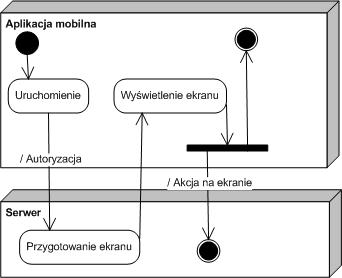
\includegraphics{img/pool_schema_uml.png} }}
\end{center}
\begin{itemize}
  \item Tworzymy nowy 'ekran' na serwerze. Oznacza to okre�lenie wygl�du i
  zachowania aplikacji w formacie XML. Okre�lamy dost�pne dla
  danego ekranu akcje. 
  \item Aplikacja mobilna ��czy si� z serwerem i pobiera przygotowany dla niej
  ekran. U�ytkownik wykonuje jedn� z dost�pnych na nim akcji, a informacja o
  tym jest przesy�ana do serwera. 
  \item Aplikacja mobilna pobiera kolejny ekran przygotowany przez serwer i
  dalej post�puje wed�ug powy�szego schematu. Poniewa� to serwer jest w ca�o�ci
  odpowiedzialny na przygotowanie ekranu, pojawia si� mo�liwo�� kontrolowania
  ekranu i jego zachowania po stronie klienta w dowolny spos�b.
\end{itemize}


\section{Mo�liwo�ci i zastosowania}
Aplikacja oparta na tak zaprojektowany model, posiada�aby cechy typowe dla
modelu dwuwarstwowego - w tym szybki czas reakcji, niezale�no�� wygl�du aplikacji od
stosowanego klienta oraz mo�liwo�� przeprowadzenia pewnych dodatkowych operacji
(jak walidacja) po stronie klienta. W idealnym przypadku m�g�by by�
dynamicznie przesy�any kod, wykonywany po stronie klienta (odpowiednik
JavaScript w przypadku przegl�darki internetowej). Pozbawiona by�aby te�
typowych wad obu rozwi�za� - brak konieczno�ci aktualizowania aplikacji przy
drobnych poprawkach (poza b��dami w zainstalowanym oprogramowaniu). Nie by�aby 
r�wnie� ograniczona do mechanizm�w, oferowanych przez statyczne strony WWW -
mo�na by by�o wy�wietla� dowolne ekrany, a na nich wykonywa� dowolne akcje.
Dodatkowo, poniewa� stan aplikacji przechowywany by�by na serwerze, mo�na by�oby
w dowolnym momencie zmieni� urz�dzenie mobilne, wy��czy� aplikacj�, a potem
powr�ci� do zapami�tanego wcze�niej miejsca.
 
\paragraph{Nowe podej�cie}
 
W przypadku tworzenia aplikacji mobilnych naturalna jest ch�� przeniesienia 
funkcjonalno�ci dost�pnych w aplikacjach na komputerach stacjonarnych, na
urz�dzenie mobilne. Nie zawsze jest to podej�cie s�uszne - u�ytkownik,
korzystaj�cy z urz�dzenia mobilnego - palmtopa czy telefonu kom�rkowego, ma
znacznie ograniczone mo�liwo�ci dzia�ania i tym, co si� w takiej sytuacji
liczy, jest szybko�� i �atwo�� obs�ugi aplikacji, kt�r� mo�na postawi� przed
jej du�ymi mo�liwo�ciami. Wobec tego, naszym zdaniem, celem tworzenia aplikacji
mobilnych nie powinno by� dostarczenie wszystkich mo�liwych funkcjonalno�ci,
ale raczej maksymalna ergonomia i prostota u�ycia. Te cele przy�wieca�y
nam w trakcie tworzenia szablonu.
\newline 
Ponadto, techniczne rozwi�zania, przyj�te w szablonie, nie by�y - zgodnie z
nasz� wiedz� - do tej pory stosowane. Nasz szablon opiera si� na bibliotece
KUIX. Jest to biblioteka umo�liwiaj�ca wykorzystanie formatu XML do budowania
interfejsu u�ytkownika. Pozwala to na dynamiczne �adowanie komponent�w wcze�niej przygotowywanych na serwerze.
Naturaln� drog� rozwoju by�oby rozbudowanie szablonu o mo�liwo�� dynamicznego
�adowania kodu, mechanizm�w walidacji czy tworzenia grafiki.

\paragraph{Zastosowania}
Opisywana idea u�atwia tworzenie okre�lonego typu aplikacji i tak, jak ka�dy
szablon nie pokrywa wszystkich istniej�cych rozwi�za�. Nasz szablon u�atwi
pisanie aplikacji nie wymagaj�cej przesy�ania du�ych ilo�ci danych i od
kt�rej oczekujemy wi�kszej interaktywno�ci ni� w przypadku strony internetowej
pozbawionej JavaScript: 
\begin{itemize}
  \item Ankietowanie. Jednym z zastosowa�, kt�re mo�emy sobie wyobrazi�, jest zdalne ankietowanie
u�ytkownik�w. Stworzenie aplikacji wy�wietlaj�cej na ekranie list�
dost�pnych odpowiedzi i pozwalaj�cej na wybranie jednej z nich, jest przy u�yciu
przedstawianego szablonu prostym zadaniem.  
	\item Zdalne podejmowanie decyzji. Podobnie jak powy�ej, u�ytkownicy mog� wybra� jedn� z mo�liwych decyzji, w
takim przypadku potrzebne b�dzie rozbudowanie szablonu o zaawansowane
mechanizmy bezpiecze�stwa, jednak idea pozostaje podobna.	
	\item Zdalne wy�wietlanie tre�ci. Urz�dzenie mobilne mo�e by� te� jedynie miejscem, kt�re wy�wietla dostarczane do
niego informacje. Interakcja z u�ytkownikiem mo�e by� w tym momencie
wy��czona, a urz�dzenie mobilne mo�e pe�ni� rol� zdalnie kontrolowanego ekranu.	
\end{itemize}



\section{Przypadki u�ycia}

\begin{center}
	\begin{tabular}{ | p{4cm} | p{9cm} | }
	\hline
 PU 1 & Uruchom aplikacj� \\ \hline \hline
Cel &  Celem jest uruchomienie aplikacji    \\ \hline
Za�o�enia & Aplikacja jest zainstalowana na urz�dzeniu mobilnym    \\ \hline
Wynik pozytywny & Aplikacja zosta�a uruchomiona i widzimy ekran startowy 
\\ \hline 
Wynik negatywny & Nie uda�o si� uruchomi� aplikacji \\ \hline
Trigger & U�ytkownik wybiera aplikacj� spo�r�d aplikacji zainstalowanych na
urz�dzeniu mobilnym \\ \hline 
Scenariusz podstawowy & \begin{tabular}{lr}
                      	  1. U�ytkownik wybiera aplikacj� \\
                      	  2. U�ytkownik widzi ekran wyboru 
                      	 \end{tabular}
                       \\ \hline
Scenariusz alternatywny & \begin{tabular}{lr}
                            2a. Nie mo�na uruchomi� aplikacji.
                          \end{tabular}    \\ \hline
Interfejs u�ytkownika &  U�ytkownik ma mo�liwo�� po��czenia si� z serwerem (PU
2) lub dokonania zmian w konfiguracji (PU 3) \\ \hline

\end{tabular}
\end{center}



\begin{center}
	\begin{tabular}{ | p{4cm} | p{9cm} | }
	\hline
 PU 2 & Po��cz z serwerem \\ \hline \hline
Cel &  Celem jest po��czenie si� z serwerem dostarczaj�cym ekrany    \\ \hline
Za�o�enia & Aplikacja jest uruchomiona    \\ \hline
Wynik pozytywny & Widzimy ekran przes�any z serwera 
\\ \hline 
Wynik negatywny & Nie uda�o si� pobra� i wy�wietli� ekranu \\ \hline
Trigger & U�ytkownik wybiera z menu po��czenie z serwerem ekran�w \\ \hline 
Scenariusz podstawowy & \begin{tabular}{p{8cm}}
                      	  1. U�ytkownik wybiera opcj� pod��czenia do serwera \\
                      	  2. Aplikacja pod��cza si� do serwera podaj�c dane
                      	  uwierzytelniaj�ce \\
                      	  3. U�ytkownik widzi ekran pobrany z serwera serwera
                      	 \end{tabular}
                       \\ \hline
Scenariusz alternatywny & \begin{tabular}{p{8cm}}
                            2a. Nie mo�na pobra� i wy�wietli� ekranu.
                          \end{tabular}    \\ \hline
Interfejs u�ytkownika & U�ytkownik widzi ekran przekazany z serwera i dalsze
akcje na nim s� uzale�nione od aplikacji serwerowej (PU 4)
\\
\hline

\end{tabular}
\end{center}



\begin{center}
	\begin{tabular}{ | p{4cm} | p{9cm} | }
	\hline
 PU 3 & Edytuj ustawienia aplikacji \\ \hline \hline
Cel &  Celem jest edycja konfiguracji aplikacji mobilnej    \\ \hline
Za�o�enia & Aplikacja jest uruchomiona    \\ \hline
Wynik pozytywny & Uda�o si� zmieni� ustawienia aplikacji 
\\ \hline 
Wynik negatywny & Nie uda�o si� zmieni� ustawie� aplikacji \\ \hline
Trigger & U�ytkownik wybiera z menu edycj� konfiguracji \\ \hline 
Scenariusz podstawowy & \begin{tabular}{p{8cm}}
                      	  1. U�ytkownik wybiera opcj� edycji konfiguracji \\
                      	  2. U�ytkownik zmienia konfiguracj� programu \\
                      	  3. U�ytkownik zapisuje ustawienia
                      	 \end{tabular}
                       \\ \hline
Scenariusz alternatywny 1 & \begin{tabular}{p{8cm}}
                            2a. Nie mo�na uruchomi� aplikacji.
                          \end{tabular}    \\ \hline
Scenariusz alternatywny 2 & \begin{tabular}{p{8cm}}
                            3a. U�ytkownik anuluje zapis wprowadzonych zmian.
                          \end{tabular}    \\ \hline
Interfejs u�ytkownika &  U�ytkownik widzi ekran na kt�rym mo�e dodawa�,
                      	  przegl�da� i edytowa� serwery ekran�w. U�ytkownik mo�e
                      	  zaznaczy� aktywny serwer ekran�w. \\ \hline

\end{tabular}
\end{center}

\begin{center}
	\begin{tabular}{ | p{4cm} | p{9cm} | }
	\hline
 PU 4 & Wybierz odpowied� na ankiet� z serwera \\ \hline \hline
Cel &  Celem jest wybranie jednej z dost�pnych akcji    \\ \hline
Za�o�enia & Aplikacja jest uruchomiona i pod��czona do serwera ekran�w   \\
\hline Wynik pozytywny & Uda�o si� dokona� wyboru spo�r�d oferowanych opcji 
\\ \hline 
Wynik negatywny & Nie uda�o si� wybra� jednej z oferowanych opcji \\ \hline
Trigger & U�ytkownik wybiera z menu jedn� z oferowanych opcji \\ \hline 
Scenariusz podstawowy & \begin{tabular}{p{8cm}}
                      	  1. U�ytkownik wybiera jedn� z oferowanych opcji \\
                      	  2. Wyb�r jest przesy�any do serwera \\
                      	  3. Serwer przesy�a kolejny ekran (PU 2) 
                      	 \end{tabular}
                       \\ \hline
Scenariusz alternatywny & \begin{tabular}{p{8cm}}
                            1a. U�ytkownik nie podejmuje �adnej akcji przez
                            zbyt d�ugi (okre�lony w konfiguracji) 
                           czas \end{tabular}   \\ \hline
Interfejs u�ytkownika &  U�ytkownik widzi dost�pne opcje i mo�e wybra� jedn� z
 nich \\
\hline

\end{tabular}
\end{center} 
\section{Architektura}


Tak, jak zosta�o to ju� wspomniane, szablon sk�ada si� z dw�ch
g��wnych cz�ci - serwerowej oraz mobilnej. Przed przej�ciem do szczeg��w
implementacyjnych, zaprezentujemy koncepcj� ca�ego systemu.

\begin{figure}[htb]
    \begin{center}
    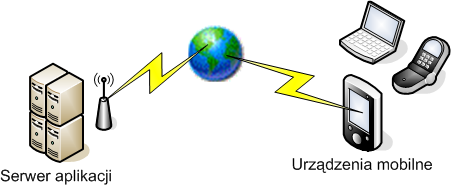
\includegraphics[angle=0,scale=0.7]{img/diag1.png}
    \end{center}
    \caption{Komunikacja mi�dzy urz�dzeniami mobilnymi i systemem enterprise}
    \label{fig:pool_arch}
\end{figure}



Jak wida�, urz�dzenia mobilne b�d� si� ��czy�y przez Internet do uruchomionego
serwera aplikacyjnego. Ka�de z nich wysy�a ��danie pobrania ekranu, kt�ry jest
dynamicznie przygotowywany w zale�no�ci od stanu aplikacji dla danego
u�ytkownika. Warto tu zwr�ci� uwag�, �e szablon jest pomy�lany w�a�ciwie
wy��cznie dla urz�dze� mobilnych - stosowane rozwi�zania s� albo niedost�pne,
albo ma�o przydatne w przypadku komputer�w stacjonarnych, o czym napiszemy
w dalszej cz�ci pracy. 
\newline
Podczas projektowania szablonu pojawi�y si� w�tpliwo�ci co do sposobu
komunikacji pomi�dzy elementami systemu. Pocz�tkowa i bardzo przekonuj�ca
koncepcja zak�ada�a wykorzystanie JMS - Java Messaging System specyfikacji
umo�liwiaj�cej przesy�anie wiadomo�ci w Javie. Przemawia� za tym szereg
argument�w:
\begin{itemize}
  \item Niezawodno�� - gwarancja dostarczenia wiadomo�ci w warunkach ��czno�ci
  bezprzewodowej szczeg�lnie nara�onej na przerwy w transmisji.
  \item Niezale�no�� system�w - u�ycie wiadomo�ci znacznie u�atwi�oby
  ewentualne zmiany po stronie serwera aplikacyjnego, ze wzgl�du na dodatkowy
  element po�rednicz�cy, jakim jest serwer wiadomo�ci.
  \item �atwo�� implementacji - przesy�ane wiadomo�ci mog� zawiera�
  zserializowane obiekty, co zdejmuje z programisty obowi�zek samodzielnej
  serializacji i deserializacji danych.
\end{itemize}
Jak si� jednak okaza�o, istotne ograniczenia techniczne po stronie urz�dze�
mobilnych uniemo�liwi�y skorzystanie z JMS. Jest to technologia wymagaj�ca
znacznych zasob�w, niedost�pnych w specyfikacji Java Micro Edition - platformy,
na kt�rej stworzyli�my nasz szablon. Nie daje ona mo�liwo�ci bezpo�redniego
pod��czenia do kana�u komunikacyjnego, co wymusza korzystanie z zewn�trznych
bibliotek. Jednak nawet wtedy okazuje si�, �e takie biblioteki korzystaj� z
Web Serwis�w jako technologii po�rednicz�cej w komunikacji. Podobnie,
automatyczna serializacja i deserializacja w takiej sytuacji nie jest jeszcze
wspierana. 
\newline
Z tych powod�w zdecydowali�my si� na wykorzystanie Web serwis�w jako warstwy
komunikacyjnej i samodzielne rozwi�zanie generowanych przez nie problem�w.

 


\subsection{Aplikacja serwerowa}

Przedstawimy teraz architektur� cz�ci serwerowej, komponenty, z kt�rych si�
sk�ada oraz wykorzystywane technologie.
\newline
Aby zrozumie� projekt ca�ego systemu, wprowad�my pewne poj�cia w naszym
systemie. Wynikaj� z nich dalsze rozwi�zania: 
\begin{itemize}
  \item \emph{Ankieta} - tre��, dla kt�rej istniej� dost�pne zdefiniowane
  odpowiedzi.
 \item \emph{Odpowied�} - jedna z mo�liwo�ci wyboru dost�pnych dla danej ankiety
  \item \emph{U�ytkownik} - konto, z kt�rym zwi�zane s� uprawnienia i udzielone
  w ankietach odpowiedzi. Jeden u�ytkownik mo�e udzieli� wielu odpowiedzi w
  trakcie dzia�ania ca�ego systemu.
\end{itemize}


Aplikacja serwerowa zbudowana zosta�a w oparciu o model tr�jwarstwowy, z
podw�jnym dost�pem (widokiem) do danych. 



\begin{figure}[htb]
    \begin{center}
    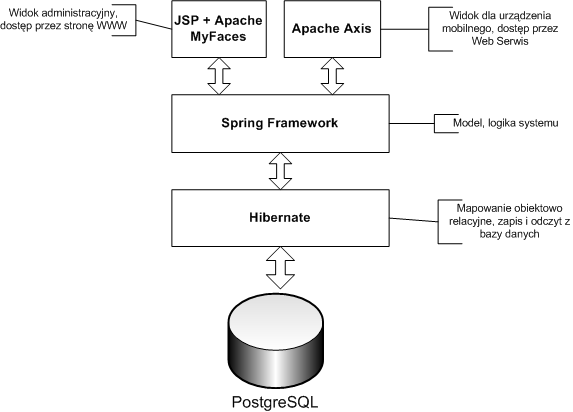
\includegraphics[angle=0,scale=0.7]{img/diag2.png}
    \end{center}
    \caption{Architektura cz�ci serwerowej szablonu integracyjnego}
    \label{fig:pool_arch2}
\end{figure}

Przedstawmy teraz poszczeg�lne warstwy systemu wraz z przyj�tymi w nich
za�o�eniami.

\paragraph{Serwer}
Aplikacja serwerowa jest uruchamiana na kontenerze Apache Tomcat 6.0.

\paragraph{Baza danych}
W oparciu o przedstawione wcze�niej za�o�enia stworzony zosta� schemat
bazy danych widoczny na rysunku \ref{fig:pool_db}.


\begin{figure}[htb]
    \begin{center}
    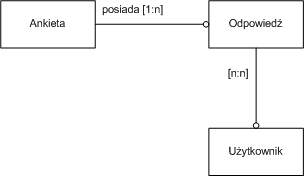
\includegraphics[angle=0,scale=0.7]{img/pool_schema_o.png}
    \end{center}
    \caption{Schemat koncepcyjny bazy danych cz�ci serwerowej szablonu
    integracyjnego}
    \label{fig:pool_db}
\end{figure}

\begin{figure}[htb]
    \begin{center}
    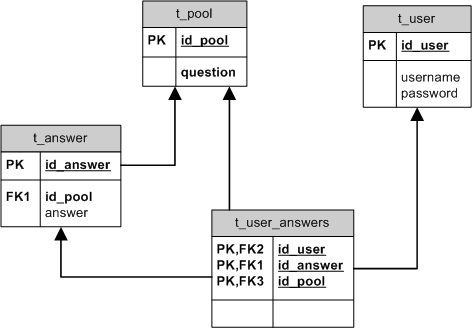
\includegraphics[angle=0,scale=0.7]{img/pool_schema.png}
    \end{center}
    \caption{Schemat fizyczny bazy danych cz�ci serwerowej szablonu
    integracyjnego}
    \label{fig:pool_db2}
\end{figure}


Schemat koncepcyjny(rysunek \ref{fig:pool_db}) jest tylko przyk�adem. Stanowi
podstaw� do prezentacji mo�liwo�ci szkieltu Kuix. Konstrukcja tego schematu mo�e
by� dowolna. Kluczowym zagadnieniem jest transformacja danych zawartych w systemie
na XML reprezentuj�cy interfejs widoczny na urz�dzeniu. Kuix jest na
tyle elastyczny, �e mo�liwe jest pod��czenie do niego dowolnego �r�d�a danych
generuj�cego XML (w szczeg�lno�ci danych nie musi dostarcza� baza relacyjna -
mo�na na przyk�ad pod��czy� baz� obiektow� Lotus Notes).
\newline
Na postawie schematu koncepcyjnego stworzony zosta� schemat fizyczny bazy
danych widoczny na rysunku \ref{fig:pool_db2}.
\newline


\index{Hibernate}
\paragraph{Hibernate}
Dost�p do danych realizowany jest za pomoc� mapowania relacyjno-obiektowego
Hibernate. Teoretycznie pozwala to, a na pewno znacznie u�atwia, ewentualn�
zmian� dostawcy bazy danych. Dodatkowo uwalnia nas z konieczno�ci r�cznego
pisania zapyta� SQL. 

\index{Spring}
\paragraph{Spring Framework}
Spring jest zestawem narz�dzi u�atwiaj�cym tworzenie aplikacji. Pozwala on
mi�dzy innymi na deklaratywne zarz�dzanie transakcjami, zarz�dzanie
cyklem �ycia obiekt�w oraz zwalnia programist� z konieczno�ci pisania
 cz�sto powtarzanego kodu przez dostarczenie odpowiednich szablon�w. Dodatkowo,
 wymusza on pewien model programowania i sprawia, �e pisane aplikacje s�
 bardziej przejrzyste i �atwiejsze w utrzymaniu. Jak ju� zosta�o wspomniane,
 aplikacja serwerowa jest aplikacj� typu Web, z kt�r� to framework Spring
 doskonale si� integruje.
 
\index{JSF}
\paragraph{Apache Myfaces} 
Myfaces jest implementacj� specyfikacji Java Server Faces pozwalaj�c� na
wygodne tworzenie widoku aplikacji. W naszym przypadku interfejsem b�dzie
dynamicznie generowana strona WWW, cho� specyfikacja JSF nie wprowadza takiego
ograniczenia. Warstwa ta b�dzie s�u�y�a do administrowania systemem,
przegl�dania podj�tych decyzji i zarz�dzania ankietami i u�ytkownikami.
\index{webserwisy}
\index{Apache Axis}
\paragraph{Apache Axis2}
Axis2 to kontener webserwis�w odpowiadaj�cy za odbieranie zdalnych wywo�a�
procedur i przekazywanie ich do mog�cych je wykona� obiekt�w.
Zwalnia programist� z konieczno�ci samodzielnego przetwarzania XML w
��daniach, umo�liwia te� automatyczn� serializacj� i deserializacj� obiekt�w
Javowych. 
\index{XSLT}
\paragraph{Transformata XSLT}
Elementem wspomagaj�cym w systemie jest transformata XSLT, wykonywana na
odpowiedziach, przesy�anych do urz�dzenia mobilnego. Jej celem jest utworzenie
widoku dla urz�dzenia mobilnego w spos�b niezale�ny od generowanej odpowiedzi.
W wyniku wywo�ania procedury generuj�cej ekran tworzony jest XML zawieraj�cy
podstawowe informacje, a nast�pnie przetwarzany jest on w opisany spos�b,
dzi�ki czemu odpowied� mo�na dowolnie modyfikowa� bez zmiany kodu aplikacji.

  

\subsection{Aplikacja mobilna}

Cech� wyr�niaj�c� podej�cie prezentowane w niniejszej pracy od typowych
rozwi�za� problemu integracji system�w enterprise jest spos�b generowania
interfejsu u�ytkownika. W typowym podej�ciu po stronie aplikacji mobilnej mamy
do czynienia z raz zdefinowanym przez programist� uk�adem oraz wygl�dem
interfejsu graficznego. Wi��e si� to bezpo�redno ze sposobem pisania aplikacji,
w kt�rym programista ma do dyspozycji gotowe komponenty UI, kt�re musz� zosta�
odpowiednio oprogramowane i wkompilowane w ko�cow� wersj� aplikacji mobilnej.
To powoduje, �e jakiekolwiek zmiany w interfejsie s� mo�liwe tylko i wy��cznie
poprzez przebudow� aplikacji. A co za tym idzie tak�e i ponowne rozprowadzenie
tak zmienionego programu. Takie podej�cie generuje dodatkowe koszty, wynikaj�ce
z potrzeby zapewnienia dostarczenia aktualnej wersji aplikacji do wszystkich
klient�w, posiadaj�cych jej star� wersj�. Cz�ciowo problem ten rozwi�zuje
podej�cie, anga�uj�ce cienkiego klienta w postaci mobilnej przegl�darki
internetowej. Zapewnia ono centralizacj� aplikacji, przez co wdro�enie nowych
wersji staje si� niemal automatyczne. Niestety, rozwi�zanie tego typu jest
cz�sto niewystarczaj�co elastyczne oraz posiada s�abo rozbudowany interfejs
u�ytkownika. 
W niniejszej pracy wykorzystane zosta�o podej�cie po�rednie, b�d�ce czym�
pomi�dzy interfejsem generowanym przez przegl�darki internetowe, a
pe�nowarto�ciowym interfejsem aplikacji mobilnych. 
\subsubsection{Dynamicznie generowany interfejs u�ytkownika}
W odr�nieniu od typowej aplikacji dost�pnej na urz�dzeniach mobilnych, nasza
aplikacja nie posiada zdefiniowanego z g�ry interfejsu u�ytkownika. Za
wyj�tkiem g��wnego ekranu, wszystkie pozosta�e s� generowane na podstawie
danych, przesy�anych z serwera. System zachowuje si� analogicznie do
przegl�darki internetowej - redeneruje znaczniki interfejsu u�ytkownika. W
odr�nieniu od rozwi�za� opartych na przegl�darce, mamy mo�liwo�� zmian w
kodzie �r�d�owym aplikacji redeneruj�cej, dzi�ki czemu, w zale�no�ci od
potrzeby, mo�emy dostosowywa� zachowanie programu do wymaga� u�ytkownika. Nasza
aplikacja nie jest ograniczona przez niemodyfikowaln� przegl�dark� internetow�.
\index{Kuix}
\subsubsection{Kuix}
Opisany w poprzednim rozdziale dynamicznie generowany interfejs jest mo�liwy do
osi�gni�cia w �rodowisku J2ME przy u�yciu pewnego, danego z g�ry, uniwersalnego
sposobu opisu wygl�du poszczeg�lnych element�w aplikacji. Ze wzgl�du na
popularno�� XML oraz wsparcie dla tego j�zyka, zar�wno po stronie urz�dze�, jak
i serwer�w, mo�na przyj��, �e w�a�nie w nim opisany zostanie interfejs
u�ytkownika. Po stronie serwera, na podstawie informacji z bazy danych, budowany
b�dzie dokument XML, ��cz�cy dane z ich sposobem wizualizacji. Po stronie
urz�dzenia mobilnego, dokument ten zostanie przetworzony przez parser XML, a
nast�pnie jego poszczeg�lne elementy zostan� zmapowane na odpowiadaj�ce im
elementy interfejsu J2ME (odpowiednio rozszerzone o dodatkowe komponenty,
niedost�pne w standardowej wersji tego �rodowiska). Opisana powy�ej procedura
zosta�a zaimplementowana w szkielecie programistycznym kuix.
\subsubsection{Cechy szkieletu Kuix}
Model programistyczny, oferowany przez szkielet Kuix, znacznie r�ni si� od
innych rozwi�za� spotykanych na platformach mobilnych. Posiada on wiele cech
charakterystycznych dla lekkiego modelu tworzenia oprogramowania mobilnego -
opartego o mobiln� przegl�dark� internetow�. Najlepsz� ilustracj� zasady
dzia�ania tego szkieletu, jest przyk�adowa aplikacja, wi�c w dalszej cz�ci
pracy zostanie przedstawiony kr�tki, przyk�adowy program, obrazuj�cy podstawowe
idee.

\paragraph{HelloKuix}

Na rysunku \ref{fig:kuix_structure} widoczna jest struktura bardzo prostego programu,
posiadaj�cego wszystkie cechy dostarczane przez szkielet Kuix.

\begin{figure}[htb]
    \begin{center}
    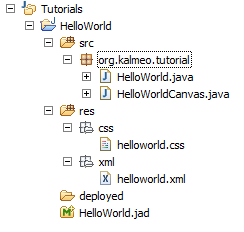
\includegraphics[angle=0,scale=0.7]{img/kuix_structure.png}
    \end{center}
    \caption{Struktura prostego projektu wykorzystuj�cego szkielet Kuix}
    \label{fig:kuix_structure}
\end{figure}


Poza standardowymi plikami *.java zawieraj�cymi kod aplikacji nale�y tu zwr�ci�
uwag� na dodatkowe pliki zasob�w :
\begin{itemize}
  \item helloworld.css
  \item helloworld.xml
\end{itemize}

Plik helloworld.xml to dokument XML we wspomnianym wcze�niej formacie,
reprezentuj�cym dane wraz ze sposobem ich wizualizacji. 

\begin{verbatim}
<screen title="helloworld">
    <container 
		style="layout:inlinelayout(false,fill); align: center">
        	<text text="Hello World!" />
        	<picture src="logo_community.png" />
    </container>
</screen>
\end{verbatim}

Tag screen to pojedynczy ekran na urz�dzeniu mobilnym, mog�cy posiada� jeden,
b�d� wi�cej, tak zwanych widget�w - element�w interfejsu u�ytkownika. Powy�szy
przyk�ad zawiera kontener (container), czyli pojemnik widget�w, pozwalaj�cy na
grupowanie ich w odr�bne uk�ady. W pojemniku znajduje si� tekst (tag text) oraz
obazek (tag picture). Informacje o zawarto�ci oraz cechach
poszczeg�lnych element�w przekazywane s� za pomoc� atrybut�w.

Powy�szy plik xml jest wczytywany na pocz�tku dzia�ania programu. S�u�y do tego
kod widoczny poni�ej.

\begin{verbatim}
// Load the content from the XML 
// file with Kuix.loadScreen static method
Screen screen = Kuix.loadScreen("helloworld.xml", null);

// Set the application current screen  
screen.setCurrent();
\end{verbatim}

Jak wida� z za��czonego przyk�adu, budowanie element�w interfejsu oraz ich
wczytywanie jest bardzo proste i w pewnien spos�b przypomina tworzenie
interfejsu u�ytkownika dla stron wy�wietlanych w przegl�darkach inernetowych.
\index{CSS}
\paragraph{CSS, a Kuix}
Charakterystycznym elementem zapo�yczonym przez Kuix z technologii
internetowych jest spos�b nadawania po��danego wygl�du elementom aplikacji.
S�u�� do tego kaskadowe arkusze styl�w (Cascading Style Sheets). W przyk��dzie
z poprzedniego paragrafu plik helloworld.css wygl�da nast�puj�co :

\begin{verbatim}
text {
    align: center;
    font-style: normal;
    color: #f19300;
}
screenTopbar text {
    color: white;
    padding: 1 2 1 2;
}
screenTopbar {
    font-style: bold;
    bg-color: #cccccc;
    border: 0 0 1 0;
    border-color: #f19300;
}
desktop {
    bg-color: #444447;
}
\end{verbatim}

Powy�szy kod CSS praktycznie niczym si� nie r�ni od tego, spotykanego w
projektach pisanych pod standardowe przegl�darki internetowe.
Do ka�dego elementu interfejsu, takiego jak ekran, czy pulpit (screen, desktop)
mamy przypisane odpowiednie selektory. Na przyk�ad, by nada� styl paskowi
tytu�owemu ekranu, u�ywamy selektora screenTopbar.

By za�adowa� do systemu plik CSS, znajudj�cy si� w zasobach projektu, nale�y
u�y� statycznej metody loadCSS klasy Kuix:

\begin{verbatim}
// Load the stylesheet from the CSS-like file with 
// Kuix.loadCss static method
//  note: a stylesheet is not associated with 
//		  a screen but with the midlet
//  note 2: by default '/css/' folder is use 
//			to find the 'helloworld.css' file
Kuix.loadCss("helloworld.css");
\end{verbatim}

Ko�cowy efekt po��czenia pliku XML ze stylami CSS widoczny jest na rysunku
\ref{fig:kuix_helloworld}.

\begin{figure}[htb]
    \begin{center}
    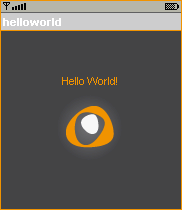
\includegraphics[angle=0,scale=0.7]{img/kuix_helloworld.png}
    \end{center}
    \caption{Wygl�d omawianej aplikacji}
    \label{fig:kuix_helloworld}
\end{figure}


W analogiczny spos�b mo�na r�wnie �atwo doda� podr�czne menu do aplikacji :

\begin{verbatim}
    <screenFirstMenu>Exit</screenFirstMenu>
    <screenSecondMenu>
        more...
        <menuPopup>
            <menuItem>
                About
            </menuItem>
            <menuItem>
                Exit
            </menuItem>
        </menuPopup>
    </screenSecondMenu> 
\end{verbatim}

Efekt ko�cowy wraz z menu dost�pnym pod prawym przyciskiem (tak zwane Second
Menu) widzimy na rysunku \ref{fig:kuix_helloworld2}

\begin{figure}[htb]
    \begin{center}
    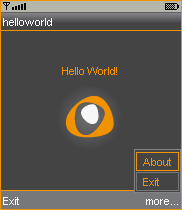
\includegraphics[angle=0,scale=0.7]{img/kuix_helloworld2.png}
    \end{center}
    \caption{Wygl�d omawianej aplikacji}
    \label{fig:kuix_helloworld2}
\end{figure}


\paragraph{Problemy}

W chwili pisania niniejszej pracy �rodowisko Kuix by�o nowo�ci� na rynku.
Najbardziej aktualna wersja 1.01 zawiera nadal du�o wad i b��d�w. Z wykonanych
przez nas test�w wynika, �e najwi�ksze problemy zwi�zane s� z pewnymi
przek�amaniami graficznymi, kt�re mo�na spotka� na urz�dzeniach mobilnych firmy
Nokia. B��dy te nie utrudnia�y pracy, a jedynie pozostawia�y wra�enie
og�lnego niedopracowania obecnej wersji szkieletu. Nale�y spodziewa� si�, �e
zostan� usuni�te w nast�pnych wersjach. 
\newline
Kolejnym powa�nym problem zwi�zanym ze szkieletem jest uboga dokumentacja
techniczna. Dobrze i szczeg�owo wykonana jest jedynie dokumentacja w
formie javadoc oraz kursy wprowadzaj�ce do tematyki. Niestety, na ich podstawie
mo�na opanowa� jedynie elementarne zasady pos�ugiwania si� �rodowiskiem. Jednak,
dzi�ki dost�pno�ci kodu �r�d�owego (Kuix jest w pe�ni otwarty), mo�liwe jest
zapoznanie si� z nieudokumentowanymi funkcjami oraz ewentualne
wprowadzenie w�asnych poprawek.
\newline
Bardzo uci��liwym problemem jest rozmiar skompilowanych bibliotek �rodowiska
Kuix. Na chwil� obecn� jest to oko�o 250 kilobajt�w. Niestety wiele urz�dze�,
w kt�re zosta�a wbudowana wirtualna maszyna Java, ogranicza dopuszczalny
rozmiar plik�w jar. Najcz�ciej ograniczenie to oscyluje w okolicach 100-150 kilobajt�w,
przez co niemo�liwe jest wykorzystanie Kuix na tych platformach. Problem ten dotyczy g��wnie rozwi�za� konsumenckich, gdy� w rozwi�zaniach mobilnych dla biznesu ograniczenia s� du�o wy�sze lub mo�liwe jest dzielenie programu na biblioteki(takie rozwi�zanie mo�na znale�� na
platformie Blackberry).

\section{Przyk�adowa implementacja: Mobilny system informacyjny}
 
Przyk�adem integracji systemu klasy Enterprise z platform� mobiln� jest
aplikacja dostarczaj�ca spersonalizowane informacje. Ide�, stoj�c� za
stworzeniem takiego systemu, jest zagospodarowanie czasu u�ytkownik�w nie
mog�cych aktywnie wyszukiwa� interesuj�cych ich wiadomo�ci. Z takimi sytuacjami mamy do czynienia
podczas oczekiwania na �rodki komunikacji miejskiej, a tak�e w czasie utrudnie�
w ruchu samochodowym. W takim momencie mo�na zaproponowa� lektur� najnowszych
informacji w skr�conej formie. Dodatkowo czytelnik w prosty spos�b mo�e
okre�li�, czy aktualnie pokazywane wiadomo�ci interesuj� go, czy te� nie. W ten
spos�b uzyskamy mo�liwo�� analizy zainteresowa� u�ytkownik�w, tak, aby w
przysz�o�ci przekazywa� im jedynie informacje, kt�re mog� ich zainteresowa�.
Ca�a aplikacja oparta jest na przedstawionym wcze�niej szablonie, do kt�rego
stworzony zosta� interfejs administracyjny, zgodny z charakterem systemu.
  
\subsection{Za�o�enia}    
Funkcjonalno�� systemu b�dzie oparta na nast�puj�cych za�o�eniach:
\begin{itemize}
  \item {Aplikacja na urz�dzeniu mobilnym wy�wietla kr�tkie,
  dostosowane do u�ytkownika informacje}
  \item {Informacje zmieniaj� si� automatycznie, tak aby ograniczy� potrzeb�
  samodzielnego ich wyszukiwania}
  \item {Istnieje mo�liwo�� okre�lenia, czy aktualnie pokazywana wiadomo�� jest
  dla nas interesuj�ca, co b�dzie mia�o wp�yw na dob�r kolejnych wiadomo�ci}
\end{itemize}

\subsection{Wymagania systemu}

\paragraph{Infrastruktura}
Potrzebne b�dzie po��czenie z Internetem, dost�pne z urz�dzenia mobilnego, jak i
z serwera, dostarczaj�cego informacje. Dodatkowo, dla komfortowego przegl�dania
wiadomo�ci, urz�dzenie mobilne powinno posiada� ekran o odpowiednio du�ej
rozdzielczo�ci (co najmniej 320x240).

\paragraph{Oprogramowanie} 
Urz�dzenie mobilne b�dzie musia�o posiada� maszyn� wirtualn� Java. Aplikacja na
serwerze b�dzie dzia�a�a pod kontrol� kontenera Apache Tomcat.

\subsection{Wst�pna analiza projektu} 
Przypuszczamy, �e system, kt�ry planujemy stworzy� mo�e znale�� realne
zastosowanie i odnie�� sukces rynkowy. 
 
\begin{center}
	\begin{tabular}{ | l | p{5cm} | p{5cm} | }
	\hline

 & Zalety & Wady \\ \hline
Wewn�trzne &  Wykorzystanie popularnej platformy & Powolna lub przerywana
transmisja \\ & Niski koszt rozwi�zania & Zbyt ma�y ekran i ma�a ergonomia
u�ytkowania
\\ 
\hline
Zewn�trzne & D�ugi czas sp�dzany w korkach lub w �rodkach komunikacji w du�ych
miastach & Obawa ludzi przed korzystaniem z internetu mobilnego, jako ci�gle
zbyt drogiego \\
& Podatno�� ludzi na kr�tkie, podane w ciekawej formie informacje& \\
\hline
\end{tabular}
\end{center}


\paragraph{Podobne systemy}
Do stworzenia tego rozwi�zania zainspirowa� nas system wy�wietlania wiadomo�ci
na stacjach i w wagonach metra. Tym, co chcieliby�my w nim udoskonali�, to
mo�liwo�� dostarczenia spersonalizowanych, dostosowanych do ka�dego czytelnika
informacji.


\subsection{Interfejs mobilny}

Mobilny klient naszej aplikacji jest midletem, zbudowanym w oparciu o szkielet
Kuix. Wersja instalacyjna sk�ada si� z dw�ch plik�w :
\begin{itemize}
  \item {Archiwum jar, zawieraj�cego midlet}
  \item {Deskryptora jad, zawieraj�cego dane niezb�dne do instalacji aplikacji w
  trybie OTA (Over-The-Air)}
\end{itemize}

\paragraph {Menu g��wne}

Po instalacji aplikacji w zak�adce, zawieraj�cej list� zainstalowanych na
telefonie midlet�w, powinna pojawi� si� nowa aplikacja o nazwie mINFO. Po jej
uruchomieniu zostaniemy przeniesieni do g��wnego ekranu, zawieraj�cego trzy
opcje :
\begin{itemize}
  \item {Show news - rozpoczyna �adowanie danych ze wskazanego serwera}
  \item {Settings - pozwala na skonfigurowanie �r�d�a danych (serwera)}
  \item {Exit - ko�czy dzia�anie midletu}
\end{itemize}

Na rysunku \ref{fig:phone_processed1} widzimy g��wne menu aplikacji. Zosta�a ona uruchomiona w
domy�lnym �rodowisku symulacyjnym, dostarczonym razem z pakietem Netbeans
Mobility Pack.

\begin{figure}[htb]
    \begin{center}
    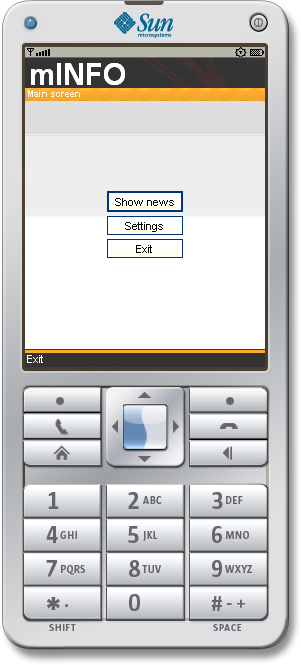
\includegraphics[angle=0,scale=0.7]{img/phone_processed1.png}
    \end{center}
    \caption{Ekran startowy aplikacji}
    \label{fig:phone_processed1}
\end{figure}


\paragraph {Zak�adka Settings}

W zak�adce settings (rysunek \ref{fig:phone_processed2}) mamy mo�liwo�� wybrania
adresu, pod kt�rym znajduje si� serwer, dostarczaj�cy dane dla naszej aplikacji. Aplikacja potrafi zapami�ta�
kilka takich adres�w. By doda� nowy adres, nale�y w polu 'New feed address'
wpisa� URL do nowego serwera, a nast�pnie wybra� przycisk 'New feed'. Je�li
chcemy pozby� si� niepotrzebnych wpis�w, znajduj�cych si� na li�cie, to
zaznaczamy wpis do usuni�cia, a nast�pnie wybieramy przycisk 'Remove feed'.
Istnieje tak�e mo�liwo�� modyfikacji adresu URL serwera. S�u�y do tego przycisk
'Edit feed'.

\begin{figure}[htb]
    \begin{center}
    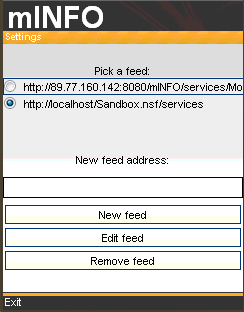
\includegraphics[angle=0,scale=0.7]{img/phone_processed2.png}
    \end{center}
    \caption{Ekran wyboru serwera wiadomo�ci}
    \label{fig:phone_processed2}
\end{figure}

Zak�adk� 'Settings' po wprowadzeniu nowego adresu
serwera widzimy na rysunku \ref{fig:phone_processed3}.

\begin{figure}[htb]
    \begin{center}
    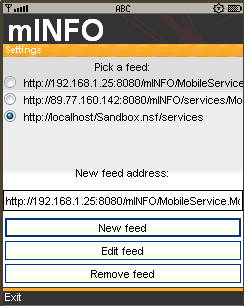
\includegraphics[angle=0,scale=0.7]{img/phone_processed3.png}
    \end{center}
    \caption{Ekran wyboru po dodaniu nowego serwera wiadomo�ci}
    \label{fig:phone_processed3}
\end{figure}


\paragraph {Dynamicznie generowane ekrany wiadomo�ci}

Po wybraniu z g��wnego menu opcji 'Show news' zostajemy zalogowani jako nowy
u�ytkownik - pod warunkiem, �e pierwszy raz pod��czamy si� do danego
serwera. W przeciwnym wypadku z pami�ci urz�dzenia zostaje odczytana uprzednio
wygenerowana nazwa u�ytkownika oraz has�o. Dzi�ki temu serwer jest w stanie
�ledzi� dzia�ania wykonywane na danym urz�dzeniu przez u�ytkownika, poddawa� je
analizie, a nast�pnie zmienia� zawarto�� wysy�anych tre�ci. Ekrany z
wiadomo�ciami s� ca�kowicie generowane po stronie serwera (nie tylko sama ich
tre��, ale tak�e elementy interfejsu u�ytkownika). Przyk�adowy ekran
informacyjny widzimy na rysunku \ref{fig:phone_processed4}.

\begin{figure}[htb]
    \begin{center}
    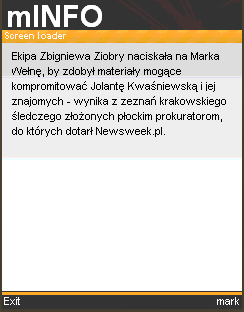
\includegraphics[angle=0,scale=0.7]{img/phone_processed4.png}
    \end{center}
    \caption{Ekran z wiadomo�ci�}
    \label{fig:phone_processed4}
\end{figure}

Ekrany s� automatycznie prze�adowywane co pewien, okre�lony z g�ry przedzia�
czasu. Dzi�ki temu, je�li u�ytkownik chce, to mo�e biernie wykorzystywa�
nasz� aplikacj� (w trybie nie wymagaj�cym interakcji). 

\paragraph {Wyb�r preferencji odno�nie tre�ci wiadomo�ci}

Je�li u�ytkownik chce wykorzystywa� aplikacj� w spos�b interaktywny, to ma do
dyspozycji podr�czne menu okre�lenia preferencji (rysunek
\ref{fig:phone_processed5}, dotycz�cych aktualnie ogl�danej wiadomo�ci. Mo�e poinformowa� system, �e dana wiadomo�� go
szczeg�lnie zainteresowa�a, lub w przeciwnym wypadku, �e nie chce wi�cej
dostawa� tego typu wiadomo�ci. Na podstawie udzielonych odpowiedzi system
personalizuje list� wiadomo�ci, kt�re zostan� wys�ane do danego u�ytkownika.
Po wybraniu preferencji zostaje natychmiast za�adowany ekran z nast�pn�
wiadomo�ci�.


\begin{figure}[htb]
    \begin{center}
    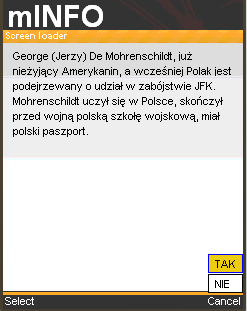
\includegraphics[angle=0,scale=0.7]{img/phone_processed5.png}
    \end{center}
    \caption{Okre�lenie preferencji u�ytkownika}
    \label{fig:phone_processed5}
\end{figure}

\begin{center}
\setlength\fboxsep{5pt}  
\setlength\fboxrule{0.0pt}
\fbox{\scalebox{0.7}{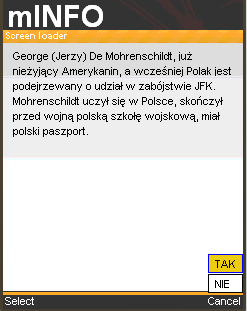
\includegraphics{img/phone_processed5.png} }}
\end{center}
\newpage
\subsection{Interfejs administracyjny}

Druga cz�� aplikacja dzia�a w kontenerze serwlet�w. Instalacja odbywa si�
poprzez umieszczenie przygotowanego archiwum w katalogu dla aplikacji. Po
przej�ciu na stron� serwletu (domy�lnie: http://serwer:port/mINFO) 
Na g�rze mamy dost�p do edycji wiadomo�ci, u�ytkownik�w oraz 'tag�w'. 
Po uruchomieniu widzimy list� wiadomo�ci (rysunek \ref{fig:server_news_list}),
znajduj�cych si� w systemie. Mo�emy dodawa� wiadomo�ci r�cznie, jak i pobra� je automatycznie z serwera
Wirtualnej Polski (dodanego g�ownie dla test�w systemu).

\begin{figure}[htb]
    \begin{center}
    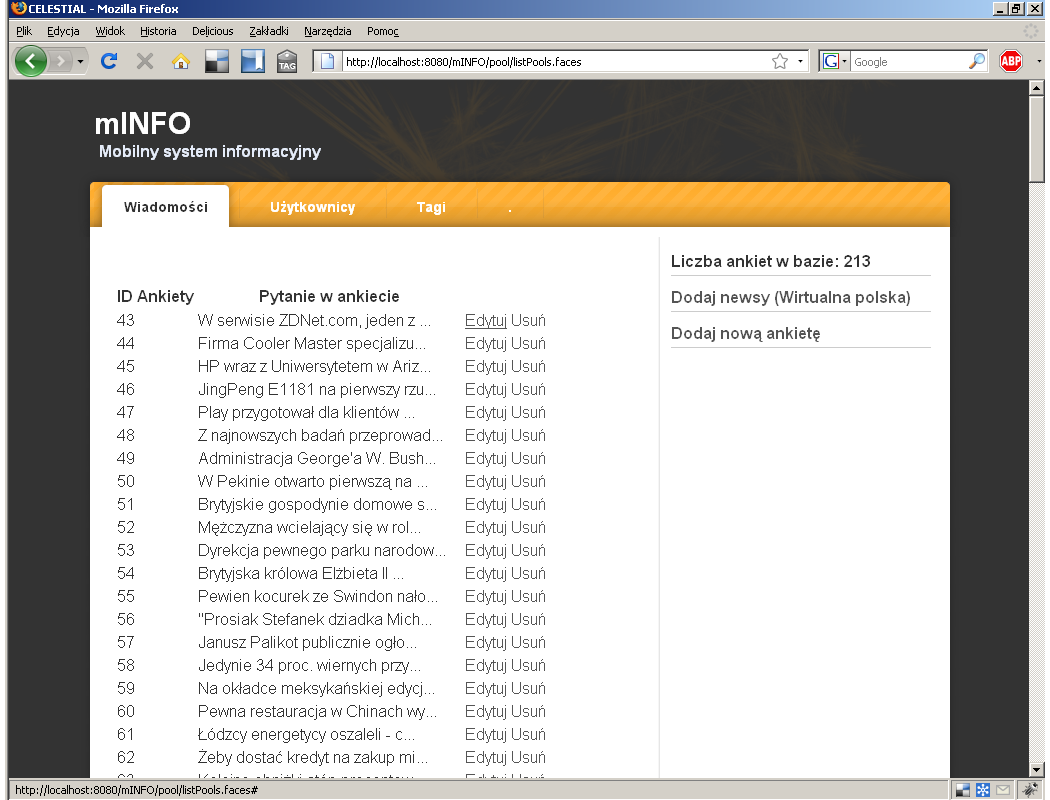
\includegraphics[angle=0,scale=0.35]{img/server_news_list.png}
    \end{center}
    \caption{Lista wiadomo�ci w systemie}
    \label{fig:server_news_list}
\end{figure}

Ka�da z wiadomo�ci jest w rzeczywisto�ci 'ankiet�', o kt�rej
wcze�niej pisali�my w opisie szablonu integracyjnego. Dost�pne odpowiedzi to
TAK i NIE, okre�laj�ce, czy dana wiadomo�� jest dla u�ytkownika interesuj�ca
(istnieje oczywi�cie mo�liwo�� dodania w�asnych odpowiedzi, jednak aplikacja,
kt�r� stworzyli�my, uwzgl�dnia tylko te dwie w dalszym przetwarzaniu). 

\begin{figure}[htb]
    \begin{center}
    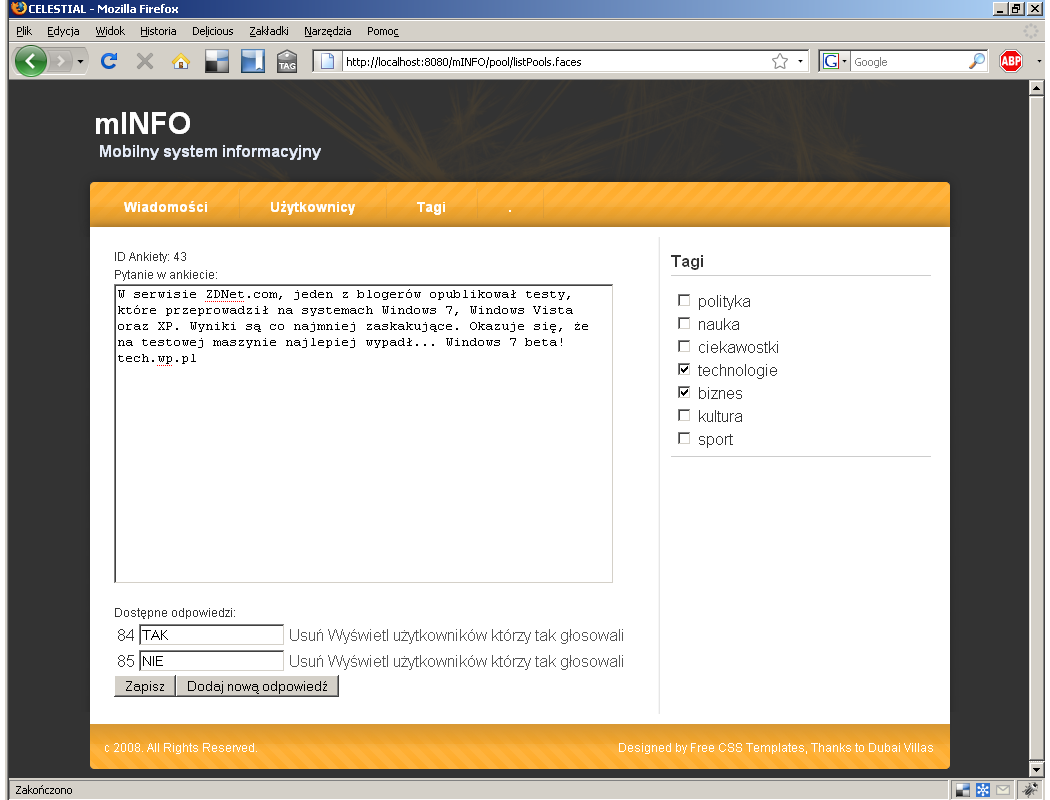
\includegraphics[angle=0,scale=0.35]{img/server_pool.png}
    \end{center}
    \caption{Edycja wiadomo�ci}
    \label{fig:server_pool}
\end{figure}


Dodatkowo, ka�d� wiadomo�� mo�emy 'otagowa�', to znaczy przypisa� j� do pewnych
kategorii tematycznych. Dzi�ki temu preferencje u�ytkownika zostaj� uog�lnione
na kategorie. Mo�emy te� obejrze� u�ytkownik�w, kt�rzy g�osowali w okre�lony
spos�b w naszej ankiecie. 
 
 \begin{figure}[htb]
    \begin{center}
    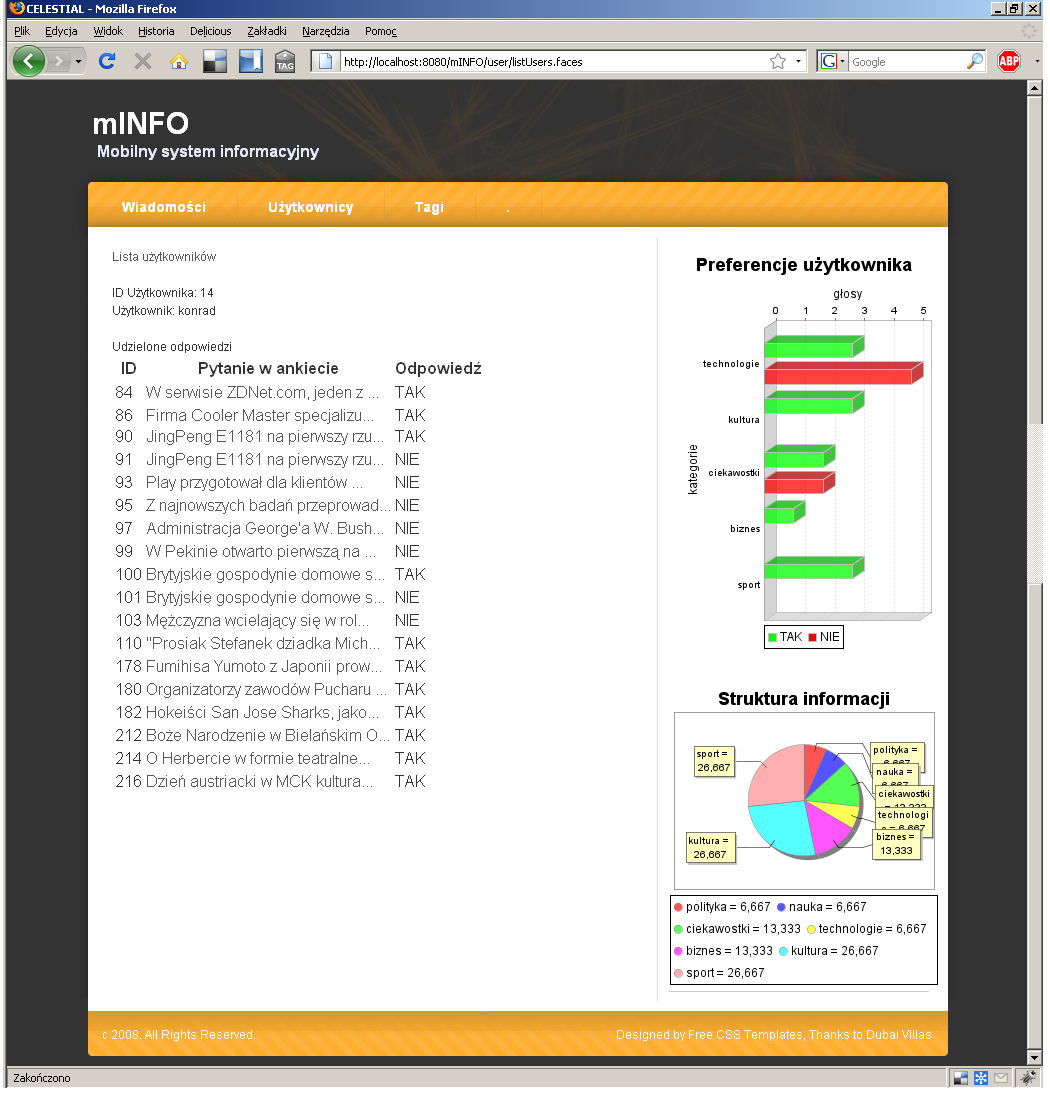
\includegraphics[angle=0,scale=0.35]{img/server_user_prefs.png}
    \end{center}
    \caption{Ustawienia i preferencje informacyjne u�ytkownika}
    \label{server_user_prefs}
\end{figure}

Na podstawie g�os�w u�ytkownika system tworzy jego profil informacyjny, aby
serwowa� mu informacje coraz bardziej odpowiadaj�ce jego zainteresowaniom.
Widzimy g�osy, kt�re odda� u�ytkownik na okre�lone kategorie oraz bierz�c�
struktur� przygotowywanych dla niego informacji. 
System na tej podstawie selekcjonuje wiadomo�ci oraz przygotowuje kolejne
ekrany informacyjne dla klienta mobilnego.
 

\chapter{Mobilny system informacyjny}


\section{Interfejs mobilny}


\section{Interfejs administracyjny}
  
 
\begin{thebibliography}{99}
\bibitem{Entj2me} Michael Juntao Yuan: \emph{Enterprise J2ME Developing Mobile
Applcations}, Prentice Hall Pennsylvania 2004
\bibitem{Entpatterns} Gregor Hophe,Bobby Woolf: \emph{Enterprise Integration
Patterns}, The Addison-Wesley Signaure Series 2003
\bibitem{j2me} Kim: Topley \emph{J2ME. Almanach}, Helion O'REILLY 2003
\bibitem{techfaq360}: \emph{Spring Tutorial},
http://www.techfaq360.com/tutorial/spring/
\bibitem{WebServicesIBM}: \emph{Which WSDL},
http://www.ibm.com/developerworks/webservices/\\library/ws-whichwsdl/
\bibitem{computerwoche} Karin Quack: \emph{Die gro�en Herausforderungen},
Computerwoche 26.03.2008
\bibitem{omapach} \emph{O mapach},
http://gps.put.mielec.pl/mapy.htm
\bibitem{operadevelop} \emph{Opera mobile - developer angle},
http://dev.opera.com/articles/view/\\opera-mobile-9-5-the-developer-angle/
\bibitem{bbdev} \emph{Java development for Blackberry},
http://na.blackberry.com/eng/developers/\\javaappdev/
\bibitem{kuix} \emph{Kuix Framework Home Page},
http://www.kalmeo.org/projects/kuix
\bibitem{j2megui} \emph{List of available GUI frameworks for Java Micro
Edition},
http://newsofthefuture.net/\\index.php?/archives/33-Evaluation-GUI-libraries-for-J2ME.html
\bibitem{bbsecurity} \emph{Blackberry security}
http://na.blackberry.com/eng/ataglance/security/\\features.jsp
\bibitem{jmsnj2me} Martin Erzberger: \emph{Using JMS and J2ME for Building
Interactive Mobile Applications}, Softwired AG, Z�rich 
\end{thebibliography} 
 
\listoffigures
 
\printindex

\appendix
 
% tutaj za��czniki

%\chapter*{Bibliografia}
%\nocite{*}
%\bibliographystyle{plplain}
%\bibliographystylebk{plplain}
%\bibliographystylest{plplain}
%\bibliographystyledoc{plplain}
% \bibliographystyleweb{plplain}
%\bibliographybk{BIB/books}
%\bibliographyst{BIB/books}
%\bibliographydoc{BIB/books}
% \bibliographyweb{BIB/books}

% \bibliography{bib/verificard,bib/jml,bib/daikon}
%\bibliography{bib/daikon,bib/statistics,bib/other}

\end{document}

% ex: set tabstop=4 shiftwidth=4 softtabstop=4 noexpandtab fileformat=unix filetype=tex encoding=utf-8 fileencodings= fenc= spelllang=pl,en spell:

%%This is a very basic article template.
%%There is just one section and two subsections.
%%\documentclass[12pt, a4paper]{report}
%%\linespread{1.5}
%%\pagestyle{headings}
%%\usepackage{fancyhdr}   
%%\usepackage{graphicx}     
%%\pagestyle{fancy}           
%zmianaliterw~ywejpaginienamae 
%%\renewcommand{\chaptermark}[1]{\markboth{#1}{}}
%%\renewcommand{\sectionmark}[1]{\markright{\thesection\ #1}}
%%\fancyhf{}%usubie�ceustawieniapagin 
%%\fancyhead[LE,RO]{\small\bfseries\thepage}
%%\fancyhead[LO]{\small\bfseries\rightmark}    
%%\fancyhead[RE]{\small\bfseries\leftmark}  
%%\renewcommand{\headrulewidth}{0.5pt}  
%%\addtolength{\headheight}{0.5pt}%pionowyodstpnakresk
%%\fancypagestyle{plain}{%  
%%\fancyhead{}%usup.g�rnenastronachpozbawionych 
%numeracji(plain) 
%%\renewcommand{\headrulewidth}{0pt}%poziomakreska
%%}
%%\usepackage{graphicx}  
%%\usepackage{polski}
%%\usepackage[cp1250]{inputenc} 
%%\end{document}
 